\documentclass{article} % For LaTeX2e
\usepackage{iclr2017_conference,times}

\usepackage{booktabs}       % professional-quality tables
\usepackage{amsfonts}       % blackboard math symbols
\usepackage{nicefrac}       % compact symbols for 1/2, etc.
\usepackage{microtype}      % microtypography
\usepackage{setspace}

\usepackage{qiangstyle}
\usepackage{url}
\newcommand{\dilinfig}{./figures}
\newcommand{\dilincheck}[1]{#1}%\textcolor{magenta}{#1}}

%\rnewcommand{\figcapsize}{\small}

\title{Learning to Draw Samples: With Application to Amortized MLE for Generative Adversarial Learning} %Training Deep Energy Models}

\author{Dilin Wang, ~~Qiang Liu\\
Department of Computer Science, Dartmouth College\\
%Institute \\
%Dartmouth College\\
\texttt{\{dilin.wang.gr, qiang.liu\}@dartmouth.edu}
}
%\author{
%Qiang Liu \& Dilin Wang \thanks{Use footnote for providing further information
%about author (webpage, alternative address)---\emph{not} for acknowledging
%funding agencies.  Funding acknowledgements go at the end of the paper.} \\
%Department of Computer Science\\
%Dartmouth College\\
%Hanover, NH 03755, USA \\
%\texttt{\{qiang.liu, XXX\}@dartmouth.edu}
%}
% The \author macro works with any number of authors. There are two commands
% used to separate the names and addresses of multiple authors: \And and \AND.
%
% Using \And between authors leaves it to \LaTeX{} to determine where to break
% the lines. Using \AND forces a linebreak at that point. So, if \LaTeX{}
% puts 3 of 4 authors names on the first line, and the last on the second
% line, try using \AND instead of \And before the third author name.

%\newcommand{\fix}{\marginpar{FIX}}
%\newcommand{\new}{\marginpar{NEW}}

%\iclrfinalcopy % Uncomment for camera-ready version


\begin{document}

\maketitle


\begin{abstract}
We propose a simple algorithm to train stochastic 
neural networks 
%black-box procedures, such as neural networks with random inputs, 
to draw samples from given target distributions for probabilistic inference. 
Our method is based on iteratively adjusting the neural network parameters 
so that the output changes along a Stein variational gradient \citep{liu2016stein} that maximumly decreases 
the KL divergence with the target distribution. 
%to decrease the KL divergence between the output random variable and the target distribution, by mimicing a recently proposed Stein variational gradient descent. 
Our method works for any target distribution specified by their unnormalized density function, 
and can train any black-box architectures that are differentiable in terms of the parameters we want to adapt. 
%By allowing to ``learn to draw samples'', our method opens a host of applications. 
%We present two examples in this paper: 
%In addition, we leverage our method to 
As an application of our method, we propose an  \emph{amortized MLE} algorithm for training deep energy model, where a neural sampler is adaptively trained to 
approximate the likelihood function. Our method mimics an adversarial game 
between the deep energy model and the neural sampler, and obtains realistic-looking images competitive with the state-of-the-art results. 
% that attempts to fool the energy model.
%by training neural samplers to approximate the gradient for maximum likelihood by training neural networks to approximate the derivative of the log partition function of unnormalized distributions
%for maximum likelihood training, % models,  
%we propose an \emph{amortized MLE} method for training deep energy model, 
%which admits an adversarial game between 
%turning the traditional MLE algorithm into a generative adversarial  
%between the deep energy model 
%and the generative neural network that attempts to fool the energy model. We show that we can get realistic-looking images competitive with the state-of-the-art results. 
%2) by treating stochastic gradient Langevin dynamics as a black-box sampler, we train to automatically adjust its learning rate to maximize its convergence speed, outperforming the hand-designed learning rate schemes. % such as adagrad. 
%generative adversarial networks. 
\end{abstract}



\section{Introduction}


Modern machine learning increasingly relies on highly complex probabilistic models to reason about uncertainty.  
A key computational challenge is to develop efficient inference techniques to approximate, or draw samples from complex distributions. 
Currently, most inference methods, including MCMC and variational inference, are hand-designed by researchers or domain experts. 
%
This makes it difficult to fully optimize the choice of different methods and their parameters, and exploit the structures in the problems of interest in an automatic way. 
%
The hand-designed algorithm can also be inefficient when it requires to make fast inference repeatedly on a large number of different distributions with similar structures. 
%
This happens, for example, when we need to reason about a number of observed datasets in settings like online learning, 
or need fast inference as inner loops for other algorithms such as maximum likelihood training. 
Therefore, it is highly desirable to develop more intelligent probabilistic inference systems that can adaptively improve its own performance to fully the optimize computational efficiency, and generalize to new tasks with similar structures. 

Specifically, denote by $p(x)$ a probability density of interest specified up to the normalization constant, which we want to draw sample from, or marginalize to estimate its normalization constant. We want to study the following problem: 

\begin{problem}\label{pro:prob1}
Given a distribution with density $p(x)$ %specified up to the normalization constant, 
and a function $f(\eta;~\xi)$ with parameter $\eta$ and random input $\xi$, 
for which we only have assess to draws of the random input $\xi$ (without knowing its true distribution $q_0$), 
and the output values of $f(\eta;~\xi)$ and its derivative $\partial_\eta f(\eta;~\xi)$ given $\eta$ and $\xi$.  
We want to find an optimal parameter $\eta$ so that the density of the random output variable $x = f(\eta;~\xi)$ with $\xi\sim q_0$ closely matches the target density $p(x)$. 
\end{problem}

Because we have no assumption on the structure of $f(\eta;~\xi)$ 
and the distribution of random input,
we can not directly calculate the actual distribution of the output random variable $x = f(\eta;~\xi)$; 
this makes it difficult to solve Problem~\ref{pro:prob1} using the traditional variational inference (VI) methods. 
Recall that traditional VI approximates $p(x)$ using simple proposal distributions $q_\eta(x)$ indexed by parameter $\eta$, 
and finds the optimal $\eta$ by minimizing KL divergence $\KL(q_\eta ~||~p) = \E_{q_\eta}[\log (q_\eta/p)]$, 
which requires to calculate the density $q_\eta(x)$ or its derivative that is not computable by our assumption 
(even when the Monte Carlo gradient estimation and the reparametrization trick \citep{kingma2013auto} are applied).  
%and hence require to calculate the density $q$ or its derivative of the random output $x = f(\eta;~\xi)$, which is unknown or difficult to calculate by our assumption. 

\begin{comment}
\begin{figure}[t]
   \centering
   \scalebox{1}{
   \includegraphics[width=.6\textwidth]{figures/neuralsampler1}%neuralbayesian} % requires the graphicx package
   }
   \begin{picture}(0,0)(0,0)
   \put(-250,-10){\figcapsize \emph{Given distribution}}
      \put(-170,-10){{\figcapsize \emph{Black-box neural sampler}}}
%      \put(-180,-10){{\figcapsize \emph{by amortized SVGD}}}      
%   \put(-180,0){\begin{tabular}{c} {\figcapsize Black-box sampler} \\[-1\baselineskip] {\figcapsize trained by amortized SVGD}    \end{tabular}}
   \put(-50,-10){\figcapsize \emph{Samples}}
   \end{picture}\\[.5em]
   \caption{\figcapsize   
   Our methods ``learn to draw samples'',  
   constructing black-box neural samplers for given distributions. 
   It allows us to automatize the hyper-parameter tuning of Bayesian inference, 
 speed up the inference inner loops of learning algorithms, 
and eventually replace hand-designed inference algorithms with more efficiently one that is trained on past tasks and is improved adaptively over time.}
% Our new amortized SVGD algorithm allows us to perform ``meta-Bayesian inference'', constructing functions that learns to produce posterior samples based on prior and data, significantly improving the efficiency of Bayesian inference at large scale.}
%   Our new amortized SVGD algorithm allows us to perform ``meta-Bayesian inference'', constructing functions that learns to produce posterior samples based on prior and data, significantly improving the efficiency of Bayesian inference at large scale.}
   \label{fig:example}
\end{figure}
\end{comment}


In fact, it is this requirement of calculating $q_\eta(x)$ 
that has been the major constraint for the designing of state-of-the-art variational inference methods with rich approximation families; 
the recent successful algorithms \citep[e.g.,][to name only a few]{rezende2015variational,tran2015variational,ranganath2015hierarchical} 
have to handcraft special variational families 
to ensure the computational tractability of $q_\eta(x)$ and simultaneously obtain high approximation accuracy, 
which require substantial mathematical insights and research effects. 
Methods that do not require to explicitly calculate $q_\eta(x)$ 
can significantly simplify the design and applications of VI methods, 
allowing practical users to focus more on choosing proposals that work best with their specific tasks. %, making the design and applications of VI much easier. 
%We should distinguish 
We will use the term \emph{wild variational inference} to refer to new variants of variational methods that require no tractability $q_\eta(x)$, %\emph{wild variational inference}, 
to distinguish with the \emph{black-box variational inference} \citep{ranganath2013black}
which refers to methods that work for generic target distributions $p(x)$ without significant model-by-model consideration (but still require to calculate the proposal density $q_\eta(x)$). 

A similar problem also appears in importance sampling (IS), 
where it requires to calculate the IS proposal density $q(x)$ in order to calculate the importance weight $w(x) = p(x)/q(x)$. 
However, %it is been shown that it is possible to develop %\emph{black-box importance sampling}  
there exist methods that use no explicit information of $q(x)$, which, seemingly counter-intuitively, give better asymptotic variance or converge rates than the typical IS that uses the proposal information \citep[e.g.,][]{liu2016black, briol2015probabilistic, henmi2007importance, delyon2014integral}.
% at least in the asymptotic sense. 
%This phoemnomin was first observed 
Discussions on this phenomenon dates back to \citet{o1987monte}, who 
argued that ``Monte Carlo (that uses the proposal information) is fundamentally unsound'' for violating the Likelihood Principle, 
and developed Bayesian Monte Carlo \citep{o1991bayes} as 
an example that uses no information on $q(x)$, yet gives better convergence rate than the typical Monte Carlo $\Od(n^{-1/2})$ rate \citep{briol2015probabilistic}. 
Despite the substantial difference between IS and VI, 
these results intuitively suggest the possibility of developing efficient variational inference without calculating $q(x)$ explicitly. 

In this work, we propose a simple algorithm for Problem~\ref{pro:prob1} 
by iteratively adjusting the network parameter $\eta$ to make its output random variable changes along 
a Stein variational gradient direction (SVGD) \citep{liu2016stein} that optimally decreases its KL divergence 
with the target distribution. 
Critically, the SVGD gradient includes a repulsive term to ensure that the generated samples have the right amount of variability that matches $p(x).$ 
In this way, we ``amortize SVGD'' using a neural network, which makes it possible for our method to adaptively improve its own efficiency  
%ccording to which shared inferences are cached and composed together to answer new queries. 
by leveraging fast experience, especially in cases when it needs to perform fast inference repeatedly on a large number of similar tasks. 
%One example of this is in maximum likelihood estimation (MLE) for unnormalized distributions, in which it is required to draw samples to approximate the likelihood at each iteration. 
%referred to as
As an application, we use our method to amortize the MLE training of deep energy models, where a neural sampler is adaptively trained to 
approximate the likelihood function. Our method, which we call \emph{SteinGAN}, mimics an adversarial game 
between the energy model and the neural sampler, and obtains realistic-looking images competitive with the state-of-the-art results produced by generative adversarial networks (GAN) \citep{goodfellow2014generative, radford2015unsupervised}. 

\paragraph {Related Work} 
The idea of amortized inference \citep{gershman2014amortized}
 has been recently applied in various domains of probabilistic reasoning, 
 including both amortized variational inference \citep[e.g.,][]{kingma2013auto, jimenez2015variational}, 
and data-driven proposals for (sequential) Monte Carlo methods \citep[e.g.,][]{paige2016inference}, 
 %and maximum a posteriori \citep{sonderby2016amortised}, 
 to name only a few. Most of these methods, however, 
 require to explicitly calculate $q(x)$ (or its gradient). 
 One exception is a very recent paper \citep{operator} that avoids calculating $q(x)$ using an idea related to Stein discrepancy \citep{gorham2015measuring, liu2016kernelized, oates2014control, chwialkowski2016kernel}.
 %; the method by \citet{operator} may be more computationally expensive than our method because it requires to train an additional neural network to distinguish $q_\eta$ and $p$ and requires to calculate the second derivative of $p(x)$. 
 There is also a raising interest recently on a similar problem of ``learning to optimize'' \citep[e.g.,][]{andrychowicz2016learning, daniel2016learning, li2016learning}, which is technically easier than the more general problem of ``learning to sample''. %that also requires to take the uncertainty into account.  
In fact, we show that our algorithm reduces to ``learning to optimize'' when only one particle is used in SVGD. 

Generative adversarial network (GAN) and its variants have recently gained remarkable success on generating realistic-looking images 
\citep{goodfellow2014generative, salimans2016improved, radford2015unsupervised, li2015generative,dziugaite2015training,nowozin2016f}.  
All these methods are set up to train latent variable models (the generator) under the assistant of the discriminator.  
Our SteinGAN instead performs traditional MLE training for a deep energy model, 
 with the help of a neural sampler that learns to draw samples from the energy model to approximate the likelihood function; 
 this admits an adversarial interpretation: we can view the neural sampler as a generator that attends to fool the deep energy model, which in turn serves as a discriminator 
that distinguishes the real samples and the simulated samples given by the neural sampler. 
This idea of training MLE with neural samplers was first discussed by \citet{kim2016deep}; 
one of the key differences is that the neural sampler in \citet{kim2016deep} 
is trained with the help of a heuristic diversity regularizer based on batch normalization, while 
SVGD enforces the diversity in a more principled way. 
%which, without a principled approach for solving Problem~\ref{pro:prob1},  in which the diversity of simulated samples are enforced with a heuristic motivated by batch normalization.  
Another method by \citet{zhao2016energy} also trains an energy score to distinguish real and simulated samples, but within a non-probabilistic framework (see Section~\ref{sec:gan} for more discussion). 
Other more traditional approaches for training energy-based models  \citep[e.g.,][]{ngiam2011learning, xie2016theory} are often based on variants of MCMC-MLE or contrastive divergence \citep{geyer1991markov, hinton2002training, tieleman2008training}, and have difficulty generating realistic-looking images from scratch. 



\section{Stein Variational Gradient Descent (SVGD)}
%This proposal will focus on integrating Stein's method with variational inference, by leveraging a new variational interpretation of Stein's characterization \eqref{equ:stein00} discovered in my recent work \citep{liu2016stein}, in which a general purpose inference algorithm called Stein variational gradient descent (SVGD) has been proposed. 
Stein variational gradient descent (SVGD) \citep{liu2016stein} is a general purpose Bayesian inference algorithm motivated by 
Stein's method \citep{stein1972, barbour2005introduction} and kernelized Stein discrepancy \citep{liu2016kernelized, chwialkowski2016kernel, oates2014control}. 
It uses an efficient \emph{deterministic} gradient-based update 
to iteratively evolve a set of particles $\{x_i\}_{i=1}^n$ to minimize the KL divergence with the target distribution. 
SVGD has a simple form that reduces to the typical gradient descent for maximizing $\log p$ when using only one particle $(n=1)$, 
and hence can be easily combined with the successful tricks for gradient optimization, 
including stochastic gradient, adaptive learning rates (such as adagrad), and momentum. % making large scale Bayesian inference both much easier and more efficient. 

To give a quick overview of the main idea of SVGD, let $p(x)$ be a positive density function on $\R^d$ which we want to 
approximate with a set of particles 
$\{ x_i\}_{i=1}^n$. 
SVGD initializes the particles by sampling from some simple distribution $q_0$, and 
updates the particles iteratively by 
%performs iterative updates of form 
\begin{align}\label{equ:xxii}
x_i  \gets x_i +  \epsilon \ff(x_i),  ~~~~ \forall i = 1, \ldots, n,  
\end{align}
where $\epsilon$ is a step size, and 
$\ff(x)$ is a ``particle gradient direction'' %  perturbation direction, or velocity field, 
%which roughly speak, is the gradient of $\KL(q_\vx~||~ p)$ w.r.t. $\vx$, 
chosen to maximumly decrease the KL divergence between the distribution of particles and the target distribution, in the sense that  
%decreases with the fastest speed in the sense that 
\begin{align}\label{equ:ff00}
\ff =   \argmax_{\ff \in \F}  \bigg\{  -   \frac{d}{d\epsilon} \KL(q_{[\epsilon\ff]} ~|| ~ p) \big |_{\epsilon = 0}  \bigg\}, 
%\frac{1}{\epsilon}\{ \KL(q_{t+1}~||~ p )  -  \KL(q_{t}~||~ p) \}, 
\end{align}
where $q_{[\epsilon \ff]}$ denotes the density of the updated particle $x^\prime = x + \epsilon \ff(x) $ when the density of the original particle $x$ is $q$, and $\F$ is the set of perturbation directions that we optimize over. 
We choose $\F$ to be the unit ball of a vector-valued reproducing kernel Hilbert space (RKHS) $\H^d = \H \times \cdots \times \H$ with each $\H$ associating with a positive definite kernel $k(x,x')$; 
%this makes $\F$
%this choice of $\F$ is broad, since $\H^d$
note that $\H$ is dense in the space of continuous functions with universal kernels such as the Gaussian RBF kernel. 
%to allow close approximation of arbitrary continuous functions. 
%which is dense in the space of continuous function with typical non-degenerate kernels such as RBF kernel. 
%We take $\F$ to be the unit ball of a reproducing kernel Hilbert space (RKHS) $\H$ associated with a positive definite kernel $k(x,x^\prime)$, 
%which can be dense in the space of continuous functions with universal (non-degenerate?) kernels such as Gaussian. 
%which is dense in the set of continuous functions when $k(x,x^\prime)$ is non-degenerate \red{(?)},  
%and also makes \eqref{equ:ff00} computationally tractable. 
%{
%{https://papers.nips.cc/paper/4168-universal-kernels-on-non-standard-input-spaces.pdf
%For example, for compact X ? Rd, [30] showed that, among a few others, the RKHSs of the Gaussian RBF kernels are universal, that is, they are dense in the space C(X) of continuous functions f : X ? R. With the help of a standard result from measure theory, see e.g. [1, Theorem 29.14], it is then easy to conclude that these RKHS are also dense in all L1(?) for which ? has a compact support. This key result has been extended in a couple of different directions: For example, [18] establishes universality for more classes of kernels on compact X ? Rd, whereas [32] shows the denseness of the Gaussian RKHSs in L1(?) for all distributions ? on Rd. Finally, [7, 8, 28, 29] show that universal kernels are closely related to so-called characteristic kernels that can be used to distinguish distributions. In addition, all these papers contain sufficient or necessary conditions for universality of kernels on arbitrary compact metric spaces X, and [32] further shows that the compact metric spaces are exactly the compact topological spaces on which there exist universal spaces.
%}

Critically, the gradient of KL divergence in \eqref{equ:ff00} 
equals a simple linear functional of $\ff$, allowing us to obtain a closed form solution for the optimal $\ff$. 
\citet{liu2016stein} showed that 
%A key observation is that the objective in \eqref{equ:ff00} is a linear functional of $\ff$, in fact, we have
\begin{align}\label{equ:klstein00}
&- \frac{d}{d\epsilon} \KL(q_{[\epsilon\ff]} ~|| ~ p) \big |_{\epsilon = 0}  = \E_{x\sim q}[\sumstein_p \ff(x)], \\[.5\baselineskip]
&~~~~\text{with}~~~~~ \sumstein_p \ff(x)  = \nabla_x \log p(x) ^\top \ff (x)+ \nabla_x \cdot \ff(x),  
\end{align}
where $\sumstein_p$ is considered as a linear operator acting on function $\ff$ and is called the Stein operator in connection with Stein's identity which shows that 
the RHS of \eqref{equ:klstein00} equals zero if $p = q$: 
\begin{align}\label{equ:steinid}
\E_{p}[\sumstein_p \ff] =\E_{p}[ \nabla_x \log p ^\top \ff + \nabla_x \cdot \ff] = 0. 
\end{align}
This is a result of integration by parts assuming the value of $p(x)\ff(x)$ vanishes on the boundary of the integration domain.   
%Obviously, $\F$ should be taken as broad as possible, best with infinite dimension, while still allows tractable solution. 
%
%Critically, we show that derivative in \eqref{equ:f00} yields a closed form representation:
%$$  \frac{d}{d\epsilon} \KL(q_{[\epsilon\ff]} ~|| ~ p) \big |_{\epsilon = 0}  = \E_{x\sim q} [\trace(\stein_p \ff(x))], $$Critically, we show that $\F$ to be the unit ball of a reproducing kernel Hilbert space (RKHS) $\H$
%
%
%%$\KL(q_{\vx^t} ~||~ p)$ between the distribution between the distribution $q_{\vx}$ of particles $\vx^t$ and the target distribution decreases with the fastest speed. 
%We take $\F$ to be the unit ball of a reproducing kernel Hilbert space (RKHS) $\H$ associated with positive definite kernel $k(x,x')$. 
%Thanks to an important connection with Stein's identity and kernelized Stein discrepancy, we show that the optimal $\phi$ is given by 
%$\ff(x)$ in RKHS $\H$ associated with positive definite kernel $k(x,x')$, in which case the optimal choice of $\ff(\vx)$ is 

Therefore, the optimization in \eqref{equ:ff00} reduces to 
\begin{align}\label{equ:ksd}
\S(q ~||~ p) \overset{def}{=} \max_{\ff \in \H^d} \{ \E_{x\sim q} [\sumstein_p \ff(x)]  ~~~s.t.~~~~ ||\ff ||_{\H^d} \leq 1\}, 
\end{align}
where $\S(q ~||~ p)$ is the kernelized Stein discrepancy defined in \citet{liu2016kernelized}, which equals zero if and only if $p = q$ under mild regularity conditions. 
Importantly, the optimal solution of \eqref{equ:ksd} yields a closed form% for the optimal solution: of \eqref{equ:ff00}:
 %Further,  it turns out that optimizing \eqref{equ:klstein00} in the unit ball of $\H$ coincides with the variational form of the kernelized Stein discrepancy in \citet{liu2016kernelized},  giving a closed form for the optimal solution of \eqref{equ:ff00}: 
$$
\ff^*(x') \propto  \E_{x\sim q}[\nabla_x \log p(x)k(x,x') + \nabla_x k(x,x')]. 
$$
%This $\ff^*$ can be treated as a gradient of the KL divergence. 
By approximating the expectation under $q$ with the empirical average of the current particles $
\{x_i\}_{i=1}^n$,  SVGD admits a simple form of update: 
\begin{align}\label{equ:update11}
%\begin{split}
%x_i ~ \gets ~ x_i  ~  + ~ \epsilon  \hat\ff^*(x_i) ~~~~~\text{where}~~~~~~ \hat \ff^*(x_i) = \hat \E_{x\in \{x_i\}} [ k(x_i, ~ x) \nabla_{x} \log p(x)  + \nabla_{x} k(x_i, x) ], 
&& &~~~~~~~~~~~ x_i ~ \gets ~ x_i  ~  + ~ \epsilon \Delta x_i, 
~~~~~~~~\forall i = 1, \ldots, n,  \notag
\\
~
&&& \text{where~~~~~}\Delta x_i = \hat \E_{x\in \{x_i\}_{i=1}^n} [  \nabla_{x} \log p(x) k(x, x_i) + \nabla_{x} k(x, x_i) ], 
%x_i ~ \gets ~ x_i  ~  + ~ \epsilon \frac{1}{n} \sum_{x\in \{x_i\}} [ k(x_i, ~ x_j) \nabla_{x} \log p(x)  + \nabla_{x} k(x_i, x) ] . 
%\end{split}
\end{align}
and $\hat\E_{x\sim \{x_i\}_{i=1}^n}[f(x)] = \sum_i f(x_i)/n$. 
The two terms in $\Delta x_i$ play two different roles: 
the term with the gradient $\nabla_x \log p(x)$ drives the particles toward the high probability regions of $p(x)$, 
while the term with $\nabla_x k(x,x_i)$ serves as a repulsive force to encourage diversity;
to see this, consider a stationary kernel $k(x,x') = k(x-x')$, then the second term reduces to $\hat \E_x \nabla_{x} k(x,x_i) = - \hat \E_x \nabla_{x_i} k(x,x_i)$, 
which can be treated as the negative gradient for minimizing the average similarity $\hat \E_x k(x,x_i)$ in terms of $x_i$. 
Overall, this particle update produces diverse points for distributional approximation and uncertainty assessment, and 
also has an interesting ``momentum'' effect in which the particles move collaboratively to escape the local optima.
%See \citet{liu2016stein} for more details. 

It is easy to see from \eqref{equ:update11} that $\Delta x_i$ reduces to the typical gradient $\nabla_x \log p(x_i)$ when there is only a single particle ($n=1$) and $\nabla_x k(x,x_i)$ when $x=x_i$,  
in which case SVGD reduces to the standard gradient ascent for maximizing $\log p(x)$ (i.e., maximum \emph{a posteriori} (MAP)). 

%This update evolves the particles collectively to match the target distribution with the two terms of $\Delta(x_i)$ playing two different roles:    the first term in $\Delta(x_i)$ is theweighted sum of the particles' gradient of the log-density, which drives the particles towards the high probability regions in a collaborative fashion; the second term can be shown to serve as a ``repulsive force'' that makes the particles repel each other to maintain a degree of diversity.
% maintaining a degree of diversity via the second term $\nabla_x k(x_i, x)$ that makes the particles repel each other.

\begin{algorithm}[t]                      % enter the algorithm environment
\caption{Amortized SVGD for Problem~\ref{pro:prob1}}% for Wild Variational Inference}          % give the algorithm a caption
\label{alg:alg1}                           % and a label for \ref{} commands later in the document
\begin{algorithmic}                    % enter the algorithmic environment
\STATE Set batch size $m$, step-size scheme $\{\epsilon_t\}$ and kernel $k(x,x')$. Initialize $\eta^0$. 
\FOR {iteration $t$}
\STATE  Draw random $\{\xi_i\}_{i=1}^m$, calculate $x_i = f(\eta^t;~\xi_i)$, 
and the Stein variational gradient $\Delta x_i$ in \eqref{equ:update11}. 
%\begin{align*}%\label{equ:dxi}
%\Delta x_i = \hat\E_{x\sim\{x_i\}_{i=1}^m} [\log p(x) k(x,x_i) + \nabla_x k(x, x_i)]. 
%\end{align*}
\STATE  Update parameter $\eta$ using \eqref{equ:follow1}, \eqref{equ:follow2} or \eqref{equ:follow3}. 
%$$\eta^{t+1} \gets \eta^{t} + \epsilon ~ \sum_{i=1}^n \partial_\eta f(\eta^t;~\xi_i)  \Delta x_i.$$ 
\ENDFOR
\end{algorithmic}
\end{algorithm}

\section{Amortized SVGD: Towards an Automatic Neural Sampler}
\label{sec:amortizedsvgd}
%\section{Our Method}

%SVGD and other particle-based methods require a large memory to store the particles when  using a large number particles. In addition, 
%Particle methods like SVGD can provide simple and consistent approximation for individual target distributions, 
SVGD and other particle-based methods become inefficient when we need to repeatedly infer
a large number different target distributions for multiple tasks, including online learning or inner loops of other algorithms, 
because they can not improve based on the experience from the past tasks, and may require a large memory to restore a large number of particles. 
We propose to ``amortize SVGD'' by training a neural network $f(\eta;~\xi)$ to mimic the SVGD dynamics, yielding a solution for Problem~\ref{pro:prob1}. 

%We propose to use a neural network $f_{\eta}$ so that the output $x = f(\eta;~\xi)$ with $\xi \sim q_0$ mimics the SVGD dynamics. 
One straightforward way to achieve this is to run SVGD to convergence and 
train $f(\eta;~\xi)$ to fit the SVGD results. 
This, however, requires to run many epochs of fully converged SVGD and can be slow in practice. 
We instead propose an \emph{incremental approach} in which $\eta$ is iteratively adjusted 
so that the network outputs $x = f(\eta;~\xi)$ changes along the Stein variational gradient direction in \eqref{equ:update11} 
in order to decrease the KL divergence between the target and approximation distribution. 
%to follow the change $\Delta x_i$ given by SVGD. 
% to mimic the SVGD updates which can summary 
%the experience from the past tasks concisely, allowing ``learning to draw samples''. 
%In this 
%Many practice applications involve a large number of target distributions with similar structures for which 
%it is inefficient to repeatedly applying SVGD or other tradition inference methods on the individual distributions separately. 
%and it would be highly desirable to intelligent systems that \emph{train itself to make better Bayesian inference over time, and also generalize well to new tasks with similar structures}. 
%becomes inefficient when we have a large number of different target distributions that requires us to run the particle algorithm repeatedly. 
%The different target
%This happens when we need to reason with different observed data or priors, or need to make iterative, real-time inference for online tasks or inner loops of learning algorithms. 
%Therefore, it is highly desirable to develop more intelligent Bayesian inference systems that can adaptively improve its own performance over time, and also generalize well to new tasks with similar structures. 

%Our idea is simple: 
%we want to iteratively adjust $\eta$ such that the black-box output $x = f(\eta;~D, \xi)$ moves along the Stein variational gradient direction $\Delta(x_i)$ in \eqref{equ:update11} in order to decrease the KL divergence between the target and approximation distribution. 
To be specific, denote by $\eta^t$ the estimated parameter at the $t$-th iteration of our method; 
each iteration of our method 
draws a batch of random inputs $\{\xi_i\}_{i=1}^m$ 
and calculate their corresponding output $x_i = f(\eta;~\xi_i)$ based on $\eta^t$; here $m$ is a mini-batch size (e.g., $m=100$). 
%as well as $x'_i  = x_i \epsilon \Delta x_i$%B
The Stein variational gradient $\Delta x_i$ in 
\eqref{equ:update11} would then ensure that $x'_i = x_i + \epsilon \Delta x_i$ forms a better approximation of the target distribution $p$. 
Therefore, we should adjust $\eta$ to make its output matches $\{x'_i\}$, 
that is, we want to update $\eta$ by
\begin{align}\label{equ:follow1}
\eta^{t+1} \gets  \argmin_\eta  \sum_{i=1}^m ||  f(\eta;~\xi_i)  - x_i' ||_2^2,  ~~~~~~ \text{where} ~~~~~~  x_i'  = x_i  + \epsilon \Delta x_i. 
\end{align}
%. 
See Algorithm~\ref{alg:alg1} for the summary of this procedure. If we assume $\epsilon$ is very small, then 
\eqref{equ:follow1} reduces to a least square optimization. To see this, note that 
$f(\eta;~\xi_i) \approx f(\eta^t;~\xi_i) + \partial_\eta f(\eta^t;~\xi_i) (\eta - \eta^t)$ by Taylor expansion. 
Since $x_i = f(\eta^t;~\xi_i)$, we have
%Therefore, 
$$
 ||  f(\eta;~\xi_i)  - x_i' ||_2^2 \approx || \partial_\eta f(\eta^t;~\xi_i) (\eta  - \eta^t)  - \epsilon \Delta x_i  ||_2^2. 
$$
%This allows us to approximate the update i
As a result, \eqref{equ:follow1} reduces to the following least square optimization: 
\begin{align}\label{equ:follow2}
\eta^{t+1} \gets \eta^t + \epsilon \Delta \eta^t, 
\text{~~~~~where~~~~~}
\Delta \eta^t = \argmin_{\delta}  \sum_{i=1}^m   || \partial_\eta f(\eta^t;~\xi_i)  \delta   -  \Delta x_i  ||_2^2. 
\end{align}
%Although $\Delta \eta^t$ can be solved with a least square optimization, 
Update \eqref{equ:follow2} can still be computationally expensive because of the matrix inversion. 
% in each iteration. 
We can derive a further approximation by performing only one step of gradient descent of \eqref{equ:follow1} (or \eqref{equ:follow2}), which gives 
\begin{align}\label{equ:follow3}
\eta^{t+1} \gets \eta^t + \epsilon  \sum_{i=1}^m   \partial_\eta f(\eta^t;~\xi_i) \Delta x_i. 
\end{align}
%based on update \eqref{equ:follow3}. 
%We find this update works efficiently in practice. It is shown in Algorithm~\ref{alg:alg1}

%In this way, everything is nice


Although update \eqref{equ:follow3} is derived as an approximation of \eqref{equ:follow1}-\eqref{equ:follow2}, 
it is computationally faster and we find it works very effectively in practice; 
this is because when $\epsilon$ is small, 
one step of gradient update can be sufficiently close to the optimum.  

%Update \eqref{equ:follow3} has a particularly 
%Intuitively speaking, 
Update \eqref{equ:follow3} also has a simple and intuitive form: \eqref{equ:follow3} can be thought as \emph{a ``chain rule'' that back-propagates the Stein variational gradient to the network parameter $\eta$}. 
%making the random sample generated by $z = f(\eta;~\xi)$ mimic the behavior of SVGD and hence move towards the target distribution. 
%Although $\Delta x_i$ is not a gradient in the typical sense, it can be interpreted as a form of functional gradient with which the update of $\eta$ can be justified theoretically. 
This can be justified by considering the special case when we use only a single particle $(n=1)$ 
in which case $\Delta x_i$ in \eqref{equ:update11} reduces to the typical gradient $\nabla_x \log p(x_i)$ of $\log p(x)$, 
%In particular, note that if we just use a single particle for each $D$, our method reduces 
and update \eqref{equ:follow3} reduces to the typical gradient ascent for maximizing 
%a typical stochastic gradient ascent for maximizing 
$$\E_{\xi}[\log p(f(\eta;~\xi))],$$  
in which case $f(\eta;~\xi)$ is trained to maximize $\log p(x)$ (that is, \emph{learning to optimize}), 
instead of \emph{learning to draw samples from $p$} for which it is crucial to use Stein variational gradient $\Delta x_i$ to diversify the network outputs. 
%instead of drawing sampling from $p$ which requires to diversify the network output. 
%the method by \citet{andrychowicz2016learning} for learning to optimize using gradient descent.

Update \eqref{equ:follow3} also has a close connection with the typical variational inference with the reparameterization trick \citep{kingma2013auto}. Let $q_\eta(x)$ be the density function of $x = f(\eta;~\xi)$, $\xi\sim q_0$. Using the reparameterization trick, the gradient of $\KL(q_\eta~||~p)$ w.r.t. $\eta$ can be shown to be 
$$
\nabla_\eta\KL(q_{\eta}~||~p) = -\E_{\xi \sim q_0}[\partial_\eta f(\eta;~\xi)(\nabla_x \log p(x) - \nabla_x \log q_\eta(x))]. 
$$
With $\{\xi_i\}$ i.i.d. drawn from $q_0$ and $x_i = f(\eta;~\xi_i), ~\forall i$, the standard stochastic gradient descent for minimizing the KL divergence is 
%can be performed by 
\begin{align}\label{equ:rep}
\eta^{t+1} \gets \eta^t +  \sum_i \partial_\eta f(\eta^t;~\xi_i) \tilde \Delta x_i, ~~~~ \text{where} ~~~~ 
\tilde \Delta x_i = \nabla_x \log p(x_i) - \nabla_x \log q_\eta(x_i). 
\end{align}
This is similar with \eqref{equ:follow3}, but replaces the Stein gradient $\Delta x_i$ defined in \eqref{equ:update11} with 
$\tilde \Delta x_i$. The advantage of using $\Delta x_i$ is that it does not require to explicitly calculate $q_\eta$,
and hence admits a solution to Problem 1 in which $q_\eta$ is not computable for complex network $f(\eta; ~\xi)$ and unknown input distribution $q_0$. 
Further insights can be obtained by noting that 
\begin{align}
\label{equ:tmp}
\Delta x_i 
& \approx \E_{x\sim q}[\nabla_x \log p(x)k(x,x_i) + \nabla_xk(x,x_i)] \notag \\
& =  \E_{x\sim q}[(\nabla_x \log p(x) - \nabla_x \log q(x))k(x,x_i)]  \\
& = \E_{x\sim q} [( \tilde \Delta x) k(x, x_i)],  \notag
%& = \E_{x\sim q} [k(x, x_i) \tilde \Delta x]  \notag
%\\&\approx  \sum_j k(x_j, x_i) \tilde \Delta x_i \notag
\end{align}
where \eqref{equ:tmp} is obtained by using Stein's identity \eqref{equ:steinid}. 
Therefore, %$\Delta x_i$ is approximately $\Delta x_i$ multiplied by a positive definite matrix $[k(x_i, x_j)]_{ij}$ and hence with positive inner product.% $\Delta x_i, \tilde \Delta x_i\la $. 
$\Delta x_i$ can be treated as a kernel smoothed version of $\tilde \Delta x_i $. 
%It is also possible to get $q_\eta(x)$-free (wild) variational inference by directly approximating $\nabla_x\log q_\eta(x)$ based on 




\section{Amortized MLE for Generative Adversarial Training}
Our method allows us to design efficient approximate sampling methods 
adaptively and automatically, and enables a host of novel applications. 
In this paper, we apply it in an amortized MLE method for training deep generative models.   
%(2) automatic hyper-parameter tuning for Bayesian inference. 
%including optimizing hyperparameters in traditional inference algorithms, 
%speeding up repeated inference tasks for online or streaming settings, or inner loops of the algorithms (such as maximum likelihood learning). 
%By leveraging state-of-the-art network architectures such as RNN and ResNet and fully optimizing the  
%or eventually replacing hand-designed infernece methods with more effiicent ones that trained on past tasks and improve adaptively over time. 

%\emph{Amortized maximum likelihood estimation (MLE) for Deep Generative Models} %Generative Adversarial Networks based
%\subsection{Amortized MLE for Generative Adversarial Training} %Generative Adversarial Networks based
 Maximum likelihood estimator (MLE) provides a fundamental approach for learning probabilistic models from data, 
but can be computationally prohibitive on distributions for which drawing samples or computing likelihood is intractable due to the normalization constant. 
Traditional methods such as MCMC-MLE use hand-designed methods (e.g., MCMC) to approximate the intractable likelihood function but do not work efficiently in practice. 
We propose to adaptively train a generative neural network to draw samples from the distribution during MLE training, which not only provides computational advantage, and also allows us to generate realistic-looking images competitive with, or better than the state-of-the-art generative adversarial networks (GAN) \citep{goodfellow2014generative, radford2015unsupervised} (see Figure~\ref{fig:mnist}-\ref{fig:facemore}).  
%See our empirical results in Figure~\ref{fig:face}.
% computationally intractable normalization constant. %(or its derivative). 

To be specific, denote by $\{x_{i,obs}\}$ a set of observed data. 
We consider the maximum likelihood training of energy-based models of form 
$$
p(x|\theta) = \exp(-\phi(x, \theta) - \Phi(\theta)), ~~~~~ \Phi(\theta) = \log \int \exp(-\phi(x,\theta))dx,
$$
where $\phi(x; ~\theta)$ is an energy function for $x$ indexed by parameter $\theta$ and $\Phi(\theta)$ is the log-normalization constant. %partition function. 
The log-likelihood function of $\theta$ is %based on maximizing the log likelihood function, 
$$
L(\theta)  =\frac{1}{n}\sum_{i=1}^n\log p(x_{i,obs} | \theta),
$$
whose gradient is %ascent update is 
\begin{align*}%
\nabla_\theta L(\theta) = -  \hat\E_{obs} [\partial_\theta \phi (x; \theta) ] +    \E_\theta [\partial_\theta \phi(x; \theta) ], 
%\nabla_\theta L(\theta) =  \la\nabla_\theta f(x; \theta) \ra_{Data} -   \la  \nabla_\theta f(x; \theta) \ra_{\theta}, 
\end{align*}
where $\hat\E_{obs}[\cdot]$ and $\E_\theta[\cdot]$ denote the empirical average on the observed data $\{x_{i,obs}\}$
and the expectation under model $p(x |\theta)$, respectively.  
The key computational difficulty is to approximate the model expectation $\E_{\theta}[\cdot]$. 
To address this problem, 
we use a generative neural network $x = f(\eta;~\xi)$ trained by Algorithm~\ref{alg:alg1} 
to approximately sample from $p(x|\theta)$, yielding a gradient update for $\theta$ of form
\begin{align}\label{equ:updatetheta}
\theta \gets \theta + \epsilon \hat\nabla_\theta L(\theta),  &\text{}& 
 \hat \nabla_\theta L(\theta) =  - \hat\E_{obs} [\partial_\theta \phi (x; \theta) ] +   \hat\E_{\eta} [\partial_\theta \phi(x; \theta) ], 
%\nabla_\theta L(\theta) =  \la\nabla_\theta f(x; \theta) \ra_{Data} -   \la  \nabla_\theta f(x; \theta) \ra_{\theta}, 
\end{align}
where $\hat \E_{\eta}$ denotes the empirical average on $\{x_i\}$ where $x_i = f(\eta;~\xi_i)$, 
$\{\xi_i\}\sim q_0$. 
As $\theta$ is updated by gradient ascent, 
$\eta$ is successively updated via Algorithm~\ref{alg:alg1} to \emph{follow} $p(x|\theta)$. 
See Algorithm \ref{alg:gan}. 

We call our method \emph{SteinGAN}, because it can be intuitively
%Our process can be 
interpreted as an adversarial game between 
the generative network $f(\eta;~\xi)$ and 
the energy model $p(x|\theta)$ which serves as a discriminator:
The MLE gradient update of $p(x|\theta)$ effectively decreases the energy of the training data and increases the energy of the simulated data from $f(\eta;~\xi)$, while the SVGD update of $f(\eta;~\xi)$ decreases the energy of the simulated data to fit better with $p(x|\theta)$.  
%Meanwhile, our procedure is still a principled maximum likelihood procedure and can be more stable than the original GAN \citep{goodfellow2014generative} that attends to find a Nash equilibrium. 
Compared with the traditional methods based on MCMC-MLE or contrastive divergence, we \emph{amortize the sampler as we train}, which gives much faster speed and simultaneously provides a high quality generative neural network that can generate realistic-looking images; see \citet{kim2016deep} for a similar idea and discussions. 
%We find that 
%Traditional approaches \citep{ngiam2011learning, xie2016theory} for training energy-based models are often based on variants of MCMC-MLE or contrastive divergence \citep{geyer1991markov, hinton2002training, tieleman2008training} can not generate realistic-looking images. 
%We will perform comprehensive tests on various applications, including image generation and semi-supervised learning. 

\begin{algorithm}[t]                      % enter the algorithm environment
\caption{Amortized MLE as Generative Adversarial Learning}% for Wild Variational Inference}          % give the algorithm a caption
\label{alg:gan}                           % and a label for \ref{} commands later in the document
\begin{algorithmic}                    % enter the algorithmic environment
\STATE {\bf Goal:} MLE training for energy model $p(x|\theta) = \exp(-\phi(x,\theta) - \Phi(\theta))$.
%the regularized likelihood $\sum_i \log \exp(-\phi(x, \theta)-\Phi(\theta)) + R(\theta)$. 
\STATE Initialize $\eta$ and $\theta$. 
\FOR {iteration $t$}
%\FOR {iteration $s$ (inner loop for updating $\eta$)}
\STATE {\bf Updating $\eta$:} Draw $\xi_i\sim q_0$, $x_i = f(\eta;~\xi_i)$; update $\eta$ using \eqref{equ:follow1}, \eqref{equ:follow2} or \eqref{equ:follow3} with $p(x)=p(x|\theta)$. Repeat several times when needed. 
%\ENDFOR
\STATE 
 {\bf Updating $\theta$:}  Draw a mini-batch of observed data $\{x_{i,obs}\}$, and simulated data $x_i = f(\eta;~\xi_i)$, update $\theta$ by \eqref{equ:updatetheta}. 
%\begin{align}\label{equ:updatetheta}
%\theta \gets \theta - \hat\E_{obs}[ \nabla_\theta \phi (x,\theta) ] + 
%\hat\E_{\eta} [\nabla_\theta \phi(x, \theta)]. % + \nabla R(\theta).  
%\end{align}
\ENDFOR
\end{algorithmic}
\end{algorithm}

\section{Experiments}
\vspace{-0.05in}

In this section, we conduct a series of experiments to evaluate our model. 
To explore whether the model learns to perform the spatial inference necessary for answering visual questions that explicitly require spatial reasoning, we design a set of experiments using synthetic visual question/answer data in Sec.~\ref{sec:synthetic1}. The experimental results of our model in standard datasets (DAQUAR~\cite{DBLP:journals/corr/MalinowskiF14} and VQA~\cite{DBLP:journals/corr/AntolALMBZP15} datasets) are reported in Sec.~\ref{sec:expstandard}.

%%%%%%%%%%%%%%%%%%%%%%%%%%%%%%%%%%%%%%%%%%%%%%%%%%%%%%%%%%%%%%%%%%%%%%%%%%%%%%%%%%%%%%%%%%%%%%%%%%%
\subsection{Exploring Attention on Synthetic Data}\label{sec:synthetic1}
%Several public datasets are available, however, 
The questions in the public VQA datasets are quite varied and difficult and often require common sense knowledge to answer (e.g., ``Does this man have 20/20 vision?'' about a person wearing glasses). Furthermore, past work~\cite{malinowski2015ask,DBLP:journals/corr/RenKZ15} showed that the question text alone (no image) is a very strong predictor of the answer.
Therefore, before evaluating on standard datasets, we would first like to
understand how the proposed model uses spatial attention to answer simple visual questions where the answer cannot be predicted from question alone. 
Our visualization demonstrates that the attention mechanism does learn to attend to objects and gather evidence via certain inference rules. 

%%%%%%%%%%% figure
\begin{figure*}[!t]
  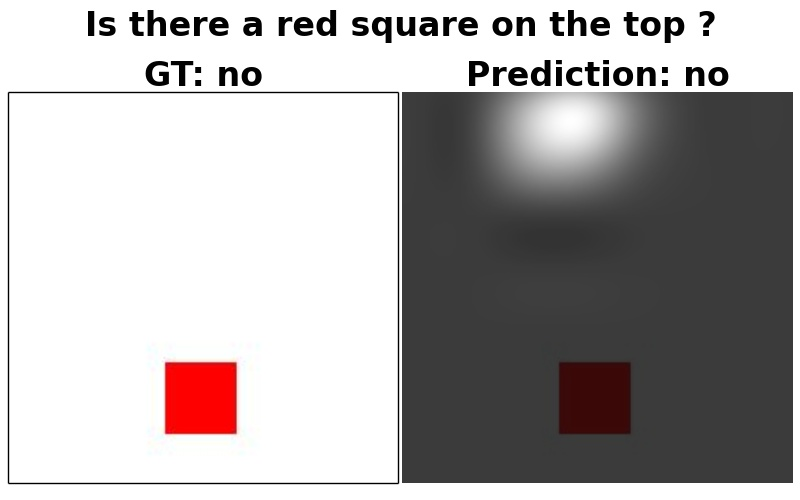
\includegraphics[width=0.242\textwidth]{figures/rule1_im_30075_219_top.JPEG}
  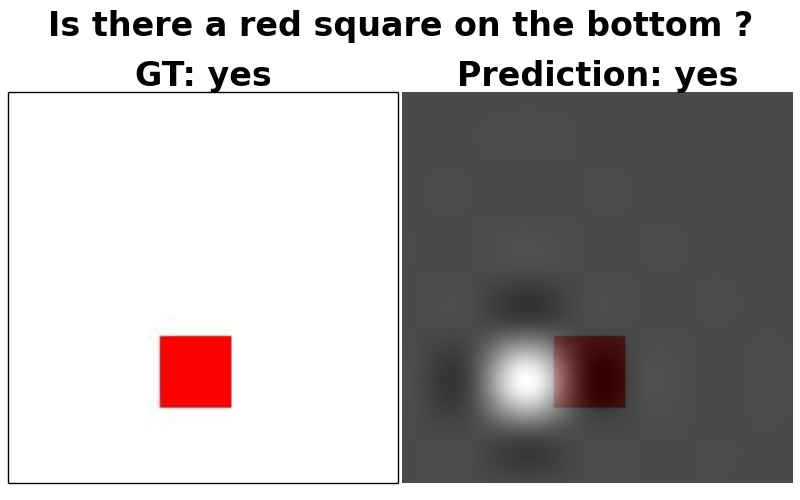
\includegraphics[width=0.242\textwidth]{figures/rule1_im_31186_4441_bottom.JPEG}
  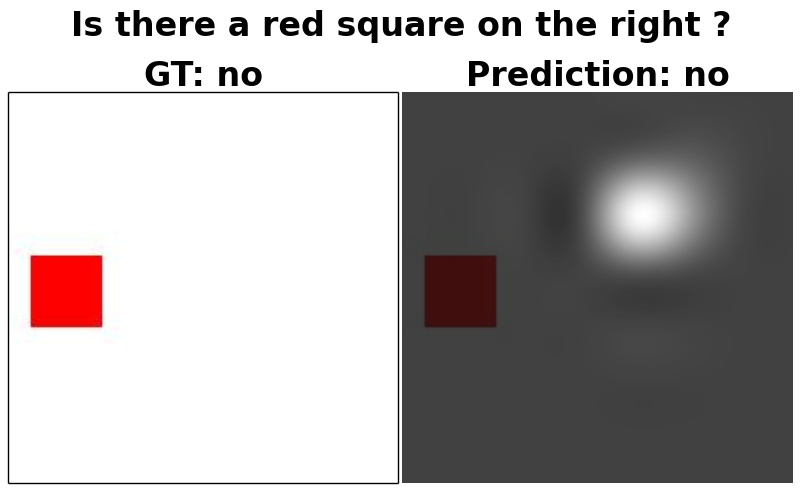
\includegraphics[width=0.242\textwidth]{figures/rule1_im_31189_690_right.JPEG}
  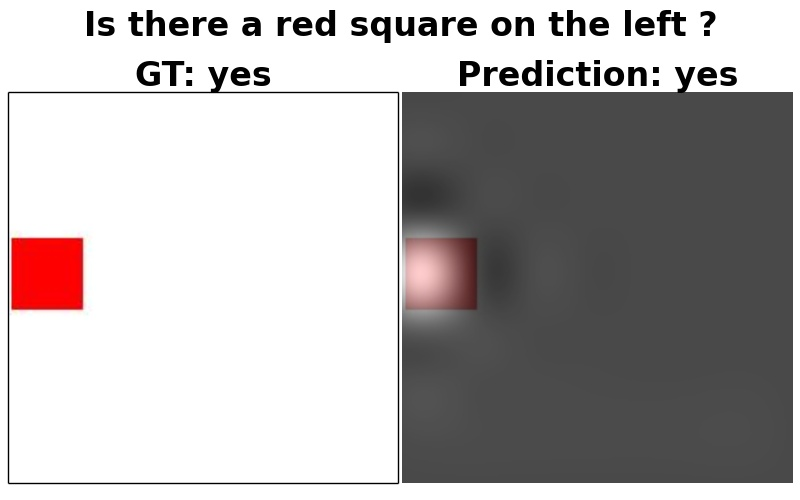
\includegraphics[width=0.242\textwidth]{figures/rule1_im_31200_4217_left.JPEG}\\
  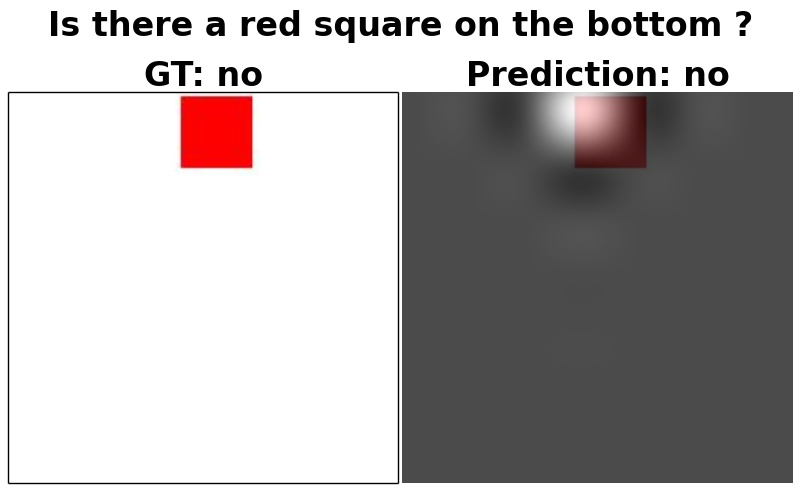
\includegraphics[width=0.242\textwidth]{figures/rule2_im_30004_3495_bottom.JPEG}
  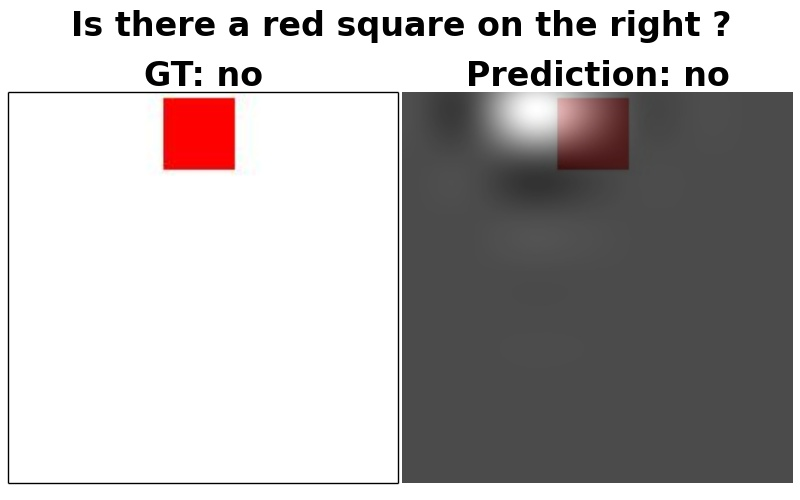
\includegraphics[width=0.242\textwidth]{figures/rule2_im_30036_3165_right.JPEG}
  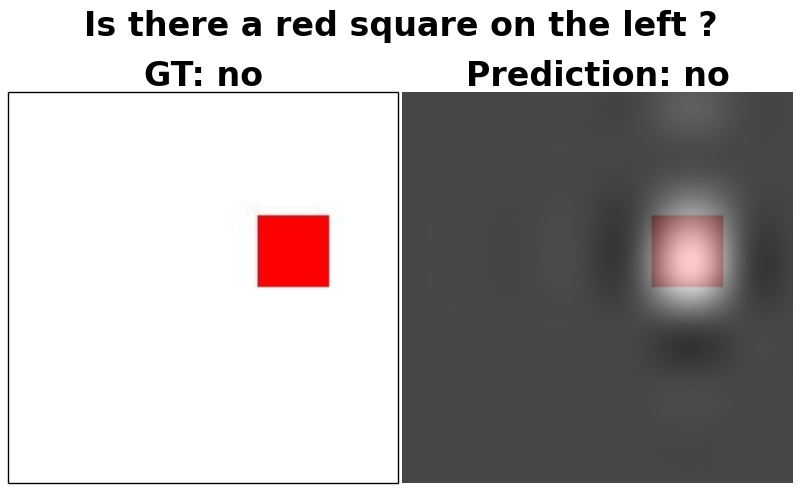
\includegraphics[width=0.242\textwidth]{figures/rule2_im_31185_2199_left.JPEG}
  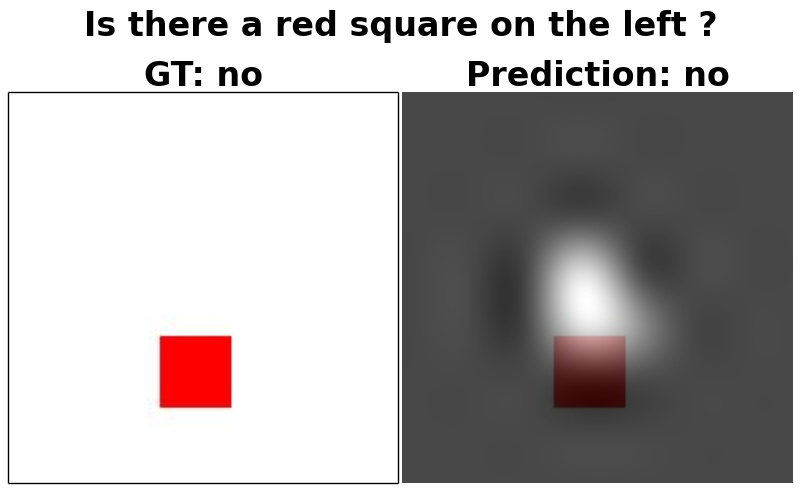
\includegraphics[width=0.242\textwidth]{figures/rule2_im_31186_1310_left.JPEG}
%\includegraphics[width=\textwidth]{figures/onehop_twohop.png}
\vspace{-0.1in}
\caption{\textbf{Absolute position experiment:} for each image and question pair, we show the original image (left) and the attention weights $W_{att}$ (right). 
The attention follows the following rules. The first rule (top row) looks at the position specified in question (top$\mid$bottom$\mid$right$\mid$left), if it contains a square, answer ``yes''; otherwise answer ``no''.
The second rule (bottom row) looks at the region where there is a square, and answers ``yes'' if the question contains that position and ``no'' for the other three positions.}\label{fig:red_square}
\vspace{-0.1in}
\end{figure*}


%%%%%%%%%%%%%%%%%%%%%%%%%%%%%%%%%%%%%%%%%%%%%%%%%%%%%%%%%%%%%%%%%%%%%%%%%%%%%%%%%%%%%%%%%%%%%%%%%%%
\vspace{-0.1in}
\subsubsection{Absolute Position Recognition}\label{sec:absolute}
We investigate whether the model has the ability to recognize the absolute location of the object in the image. We explore this by designing a simple task where an object (a red square) appears in some region of a white-background image, and the question is ``Is there a red square on the [top$\mid$bottom$\mid$left$\mid$right]?'' For each image, we randomly place the square in one of the four regions, and generate the four questions above, together with three ``no'' answers and one ``yes'' answer. The generated data is split into training and testing sets. 

Due to the simplicity of this synthetic dataset, the SMem-VQA one-hop model achieves 100\% test accuracy. However, the baseline model (iBOWIMG)~\cite{zhou2015simple} cannot infer the answer and only obtains accuracy of around 75\%, which is the prior probability of the answer ``no'' in the training set. The SMem-VQA one-hop model is equivalent to the iBOWIMG model if the attention weights in our one-hop model are set equally for each location, since the iBOWIMG model uses the mean pool of the convolutional feature ($inception\_5b/output$) in GoogLeNet that we use in SMem-VQA model. 
We check the visualization of the attention weights and find that the relationship between the high attention position and the answer can be expressed by logical expressions.
We show the attention weights of several typical examples in Fig.~\ref{fig:red_square} which reflect two logic rules:
1)~Look at the position specified in question (top$\mid$bottom$\mid$right$\mid$left), if it contains a square, then answer ``yes''; if it does not contain a square, then answer ``no''.
2)~Look at the region where there is a square, then answer ``yes'' for the question about that position and ``no'' for the questions about the other three positions.

In the iBOWIMG model, the mean-pooled GoogLeNet visual features lose spatial information and thus cannot distinguish images with a square in different positions. On the contrary, our SMem-VQA model can pay high attention to different regions according to the question, and generate an answer based on the selected region, using some learned inference rules.
This experiment demonstrates that the attention mechanism in our model is able to make absolute spatial location inference based on the spatial attention. 


%%%%%%%%%%% figure
\begin{figure*}[t]
  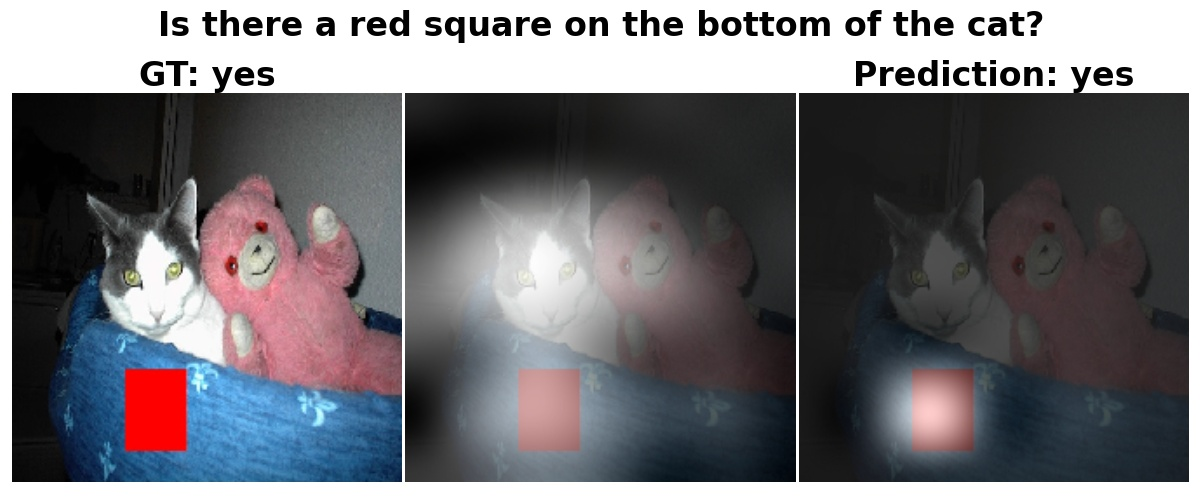
\includegraphics[width=0.325\textwidth]{figures/bottom_COCO_val2014_000000167602_bottom.jpg}
  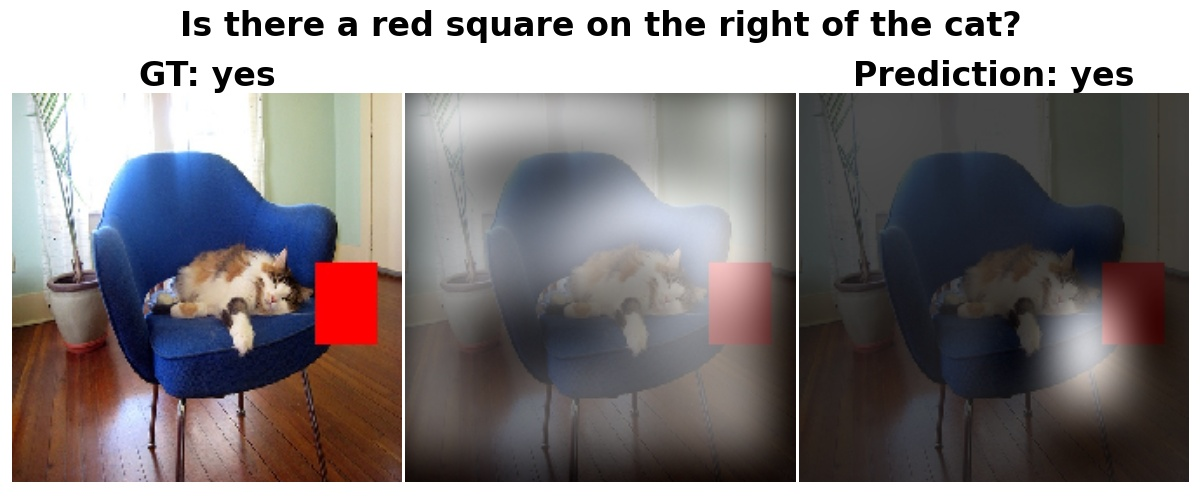
\includegraphics[width=0.325\textwidth]{figures/right_COCO_val2014_0000002988_right.jpg}
  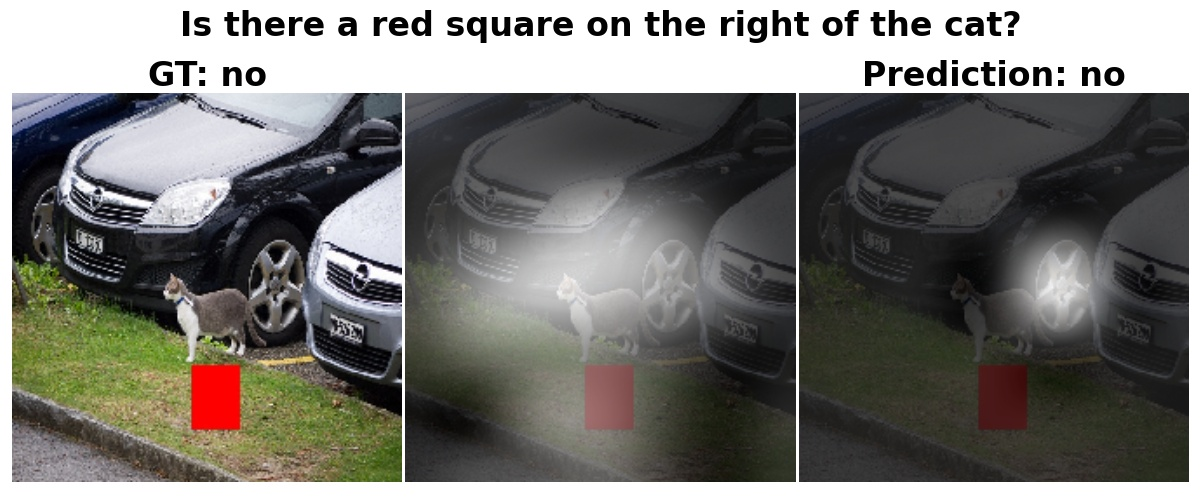
\includegraphics[width=0.325\textwidth]{figures/right_COCO_val2014_000000172330_bottom.jpg}\\
  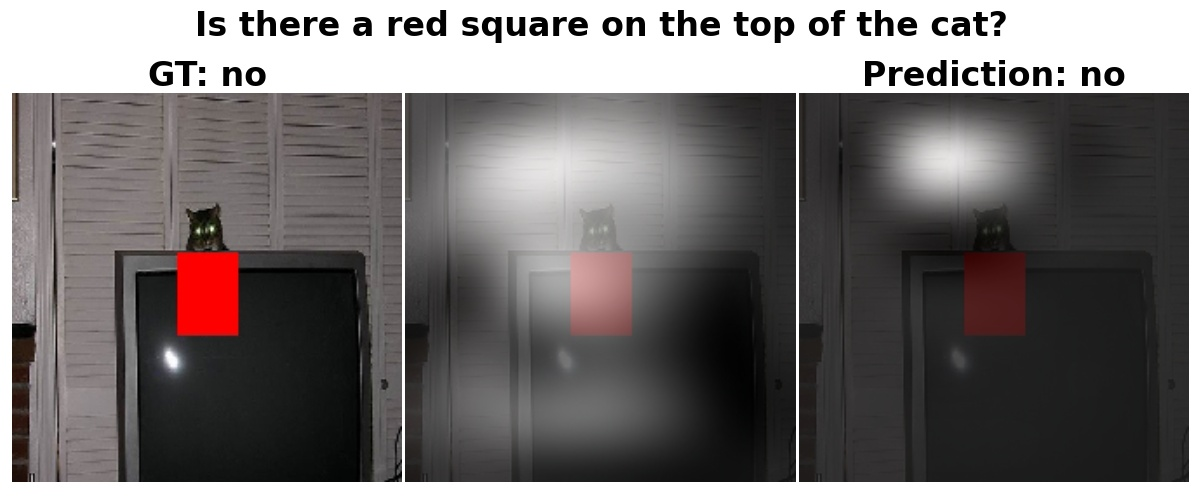
\includegraphics[width=0.325\textwidth]{figures/top_COCO_val2014_00000010694_bottom}
  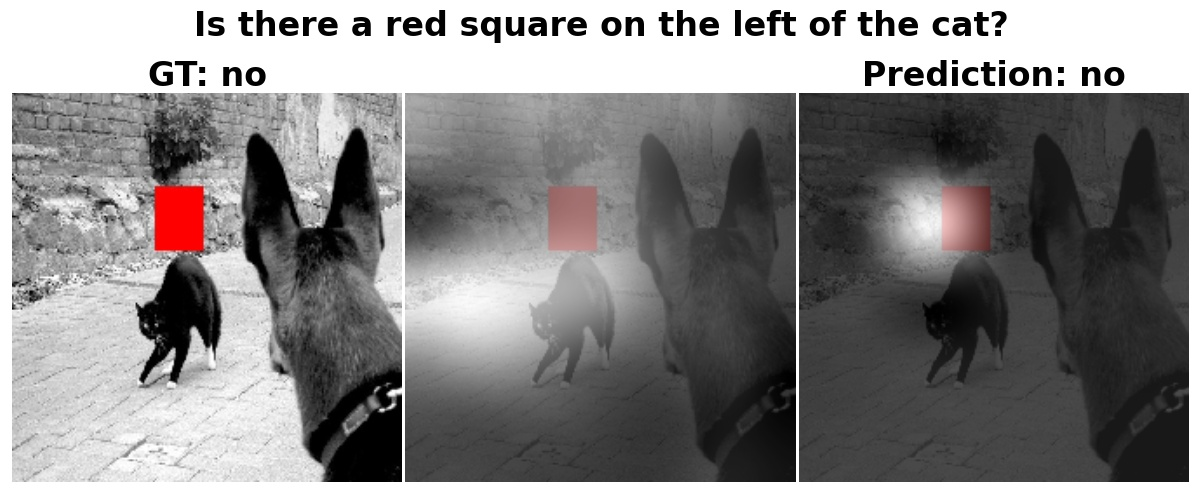
\includegraphics[width=0.325\textwidth]{figures/left_COCO_val2014_000000201918_top.jpg}
  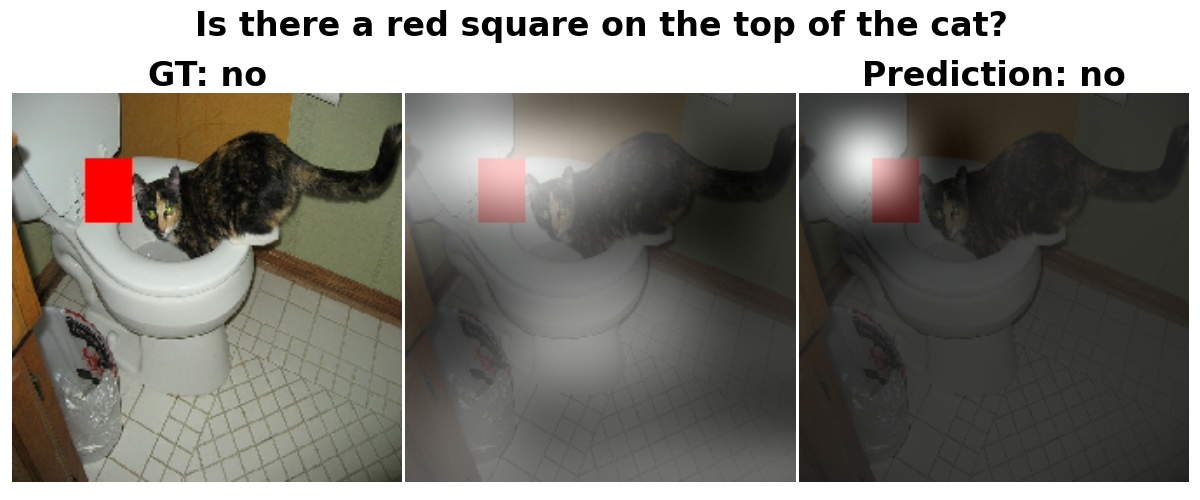
\includegraphics[width=0.325\textwidth]{figures/top_COCO_val2014_000000218924_left.jpg}
\vspace{-0.05in}
\caption{\textbf{Relative position experiment:}
for each image and question pair, we show the original image (left), the evidence embedding $W_E$ of the convolutional layer (middle) and the attention weights $W_{att}$ (right). The evidence embedding $W_E$ has high activations on both cat and red square. 
The attention weights follow similar inference rules as in Fig.~\ref{fig:red_square}, with the difference that the attention position is around the cat.
%Rule#1: (top row) look at the specified position (top/bottom/right/left), if it contains a square, answer "yes"; otherwise answer "no".
%Rule#2: (bottom row) look at the region where there is a square, answer "yes" if the question contains that position and "no" if it contains one of the other three positions.
}\label{fig:cat_square}
\vspace{-0.2in}
\end{figure*}


%%%%%%%%%%%%%%%%%%%%%%%%%%%%%%%%%%%%%%%%%%%%%%%%%%%%%%%%%%%%%%%%%%%%%%%%%%%%%%%%%%%%%%%%%%%%%%%%%%%
\vspace{-0.1in}
\subsubsection{Relative Position Recognition}
In order to check whether the model has the ability to infer the  position of one object \textit{relative} to another object,
we collect all the cat images from the MS COCO Detection dataset~\cite{lin2014microsoft}, and add a red square on the [top$\mid$bottom$\mid$left$\mid$right] of the bounding box of the cat in the images.
For each generated image, we create four questions, ``Is there a red square on the [top$\mid$bottom$\mid$left$\mid$right] of the cat?'' together with three ``no'' answers and one ``yes'' answer. 
We select 2639 training cat images and 1395 testing cat images from MS COCO Detection dataset. 

Our SMem-VQA one-hop model achieves 96\% test accuracy on this synthetic task, while the baseline model (iBOWIMG) accuracy is around 75\%.
We also check that another simple baseline that predicts the answer based on the absolute position of the square in the image gets around 70\% accuracy. 
We visualize the evidence embedding $W_E$ features and the attention weights $W_{att}$ of several typical examples in Fig.~\ref{fig:cat_square}.
The evidence embedding $W_E$ has high activations on the cat and the red square, while the attention weights pay high attention to certain locations around the cat.
We can analyze the attention in the correctly predicted examples using the same rules as in absolute position recognition experiment. 
These rules still work, but the position is relative to the cat object:
1)~Check the specified position relative to the cat, if it finds the square, then answer ``yes'', otherwise ``no''; 2)~Find the square, then answer ``yes'' for the specified position, and answer ``no'' for the other positions around the cat.
We also check the images where our model makes mistakes, and find that the mistakes mainly occur in images with more than one cats. The red square appears near only one of the cats in the image, but our model might make mistakes by focusing on the other cats.
We conclude that our SMem-VQA model can infer the relative spatial position based on the spatial attention around the specified object, which can also be represented by some logical inference rules. 



%%%%%%%%%%%%%%%%%%%%%%%%%%%%%%%%%%%%%%%%%%%%%%%%%%%%%%%%%%%%%%%%%%%%%%%%%%%%%%%%%%%%%%%%%%%%%%%%%%%
%%%%%%%%%%%%%% table
\begin{table}[!t]
\centering
\caption{Accuracy results on the DAQUAR dataset (in percentage).}
\small
 \begin{tabular}{l || c c c} 
 \hline
 ~ & DAQUAR\\ \hline
 Multi-World~\cite{DBLP:journals/corr/MalinowskiF14} & 12.73 \\ %\hline
 Neural-Image-QA~\cite{malinowski2015ask} & 29.27  \\ %\hline
 Question LSTM~\cite{malinowski2015ask} & 32.32 \\ %\hline
 VIS+LSTM~\cite{DBLP:journals/corr/RenKZ15} & 34.41 \\ %\hline
 Question BOW~\cite{DBLP:journals/corr/RenKZ15} & 32.67 \\ %\hline
 IMG+BOW~\cite{DBLP:journals/corr/RenKZ15} & 34.17 \\ \hline
 %2-VIS+BLSTM ~\cite{DBLP:journals/corr/RenKZ15} &  - & 35.78  & -\\ \hline \hline
 %Question One-Hop & 53.37 & 36.03 & - \\ %\hline   
 SMem-VQA One-Hop & 36.03 \\ %\hline   
 SMem-VQA Two-Hop & \bf{40.07} \\ \hline 
 %one dimension convolution hierarchy model\cite{ma2015learning} &  - & 0.3933 \cite{ma2015learning} & - \\ \hline
 \end{tabular}
\label{fig:baseline}
\vspace{-0.2in}
\end{table}


\subsection{Experiments on Standard Datasets}\label{sec:expstandard}
%\vspace{-0.08in}
\subsubsection{Results on DAQUAR}
The DAQUAR dataset is a relatively small dataset which builds on the NYU Depth Dataset V2~\cite{Silberman:ECCV12}. We use the reduced DAQUAR dataset~\cite{DBLP:journals/corr/MalinowskiF14}. The evaluation metric for this dataset is 0-1 accuracy. 
The embedding dimension is 512 for our models running on the DAQUAR dataset. 
We use several reported models on DAQUAR as baselines, which are listed below:\\
%\noindent
{$\bullet$} {\bf{Multi-World}}~\cite{DBLP:journals/corr/MalinowskiF14}: an approach based on handcrafted features using a semantic parse of the question and scene analysis of the image combined in a latent-world Bayesian framework.\\ 
{$\bullet$} {\bf{Neural-Image-QA}}~\cite{malinowski2015ask}: uses an LSTM to encode the question and then decode the hidden information into the answer. The image CNN feature vector is shown at each time step of the encoding phase.\\
{$\bullet$} {\bf{Question LSTM}}~\cite{malinowski2015ask}: only shows the question to the LSTM to predict the answer without any image information.\\
{$\bullet$} {\bf{VIS+LSTM}}~\cite{DBLP:journals/corr/RenKZ15}: similar to Neural-Image-QA, but only shows the image features to the LSTM at the first time step, and the question in the remaining time steps to predict the answer.\\
{$\bullet$} {\bf{Question BOW}}~\cite{DBLP:journals/corr/RenKZ15}: only uses the BOW question representation and a single hidden layer neural network to predict the answer, without any image features.\\
{$\bullet$} {\bf{IMG+BOW}}~\cite{DBLP:journals/corr/RenKZ15}: concatenates the BOW question representation with image features, and then uses a single hidden layer neural network to predict the answer. This model is similar to the iBOWIMG baseline model in~\cite{zhou2015simple}.

Results of our SMem-VQA model on the DAQUAR dataset and the baseline model results reported in previous work are shown in Tab.~\ref{fig:baseline}. 
From the DAQUAR result in Tab.~\ref{fig:baseline}, we see that models based on deep features significantly outperform the Multi-World approach based on hand-crafted features. Modeling the question only with either the LSTM model or Question BOW model does equally well in comparison, indicating the the question text contains important prior information for predicting the answer. Also, on this dataset, the VIS+LSTM model achieves better accuracy than Neural-Image-QA model; the former shows the image only at the first timestep of the LSTM, while the latter does so at each timestep. In comparison, both our One-Hop model and Two-Hop spatial attention models outperform the IMG+BOW, as well as the other baseline models.
A major advantage of our model is the ability to visualize the inference process in the deep network. To illustrate this, two attention weights visualization examples in SMem-VQA One-Hop and Two-Hop models on DAQUAR dataset are shown in Fig.~\ref{fig:2hopVQA} (bottom row).



%%%%%%%%%%% figure
\begin{figure*}[t]
%  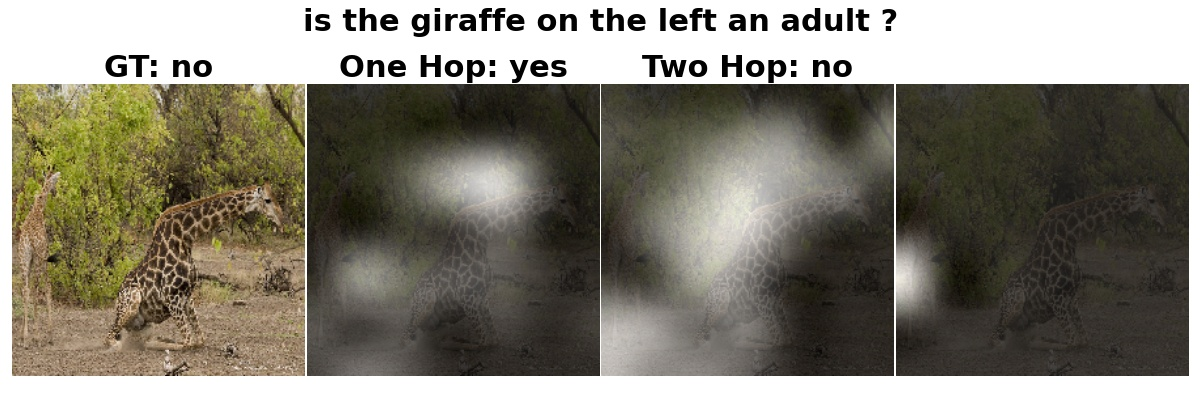
\includegraphics[width=0.5\textwidth]{figures/VQA-DAQUAR_One-Hop_Two-Hop/COCO_val2014_000000014271.jpg}
%  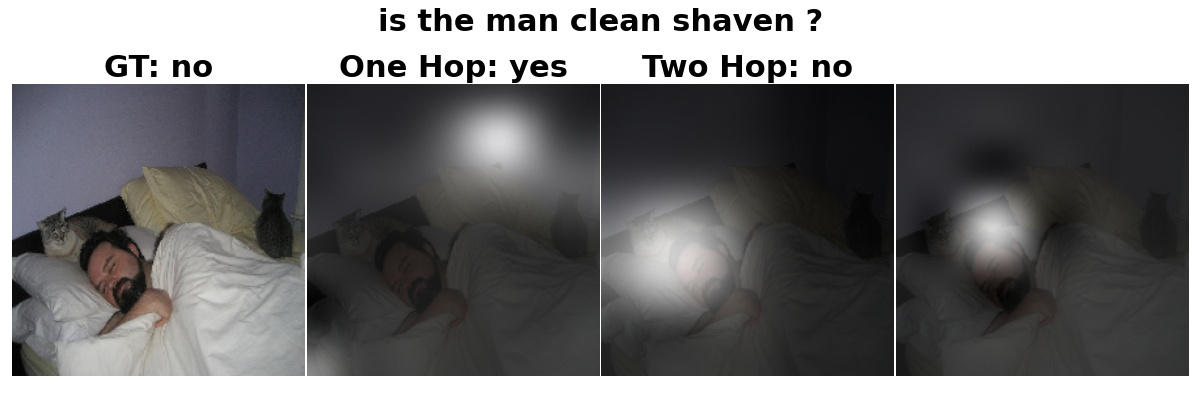
\includegraphics[width=0.5\textwidth]{figures/VQA-DAQUAR_One-Hop_Two-Hop/COCO_val2014_000000012085.jpg}\\
  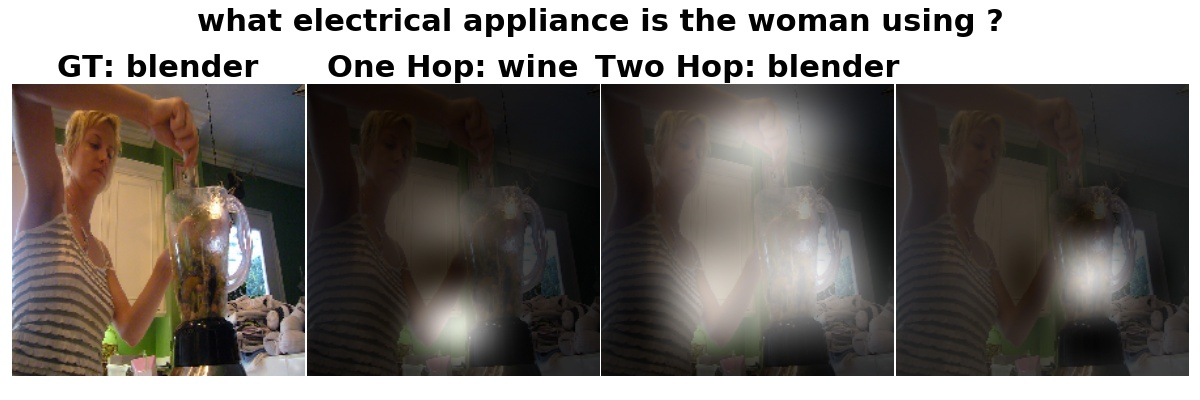
\includegraphics[width=0.5\textwidth]{figures/VQA-DAQUAR_One-Hop_Two-Hop/CO_train2014_000000575060_5750602.jpg}
  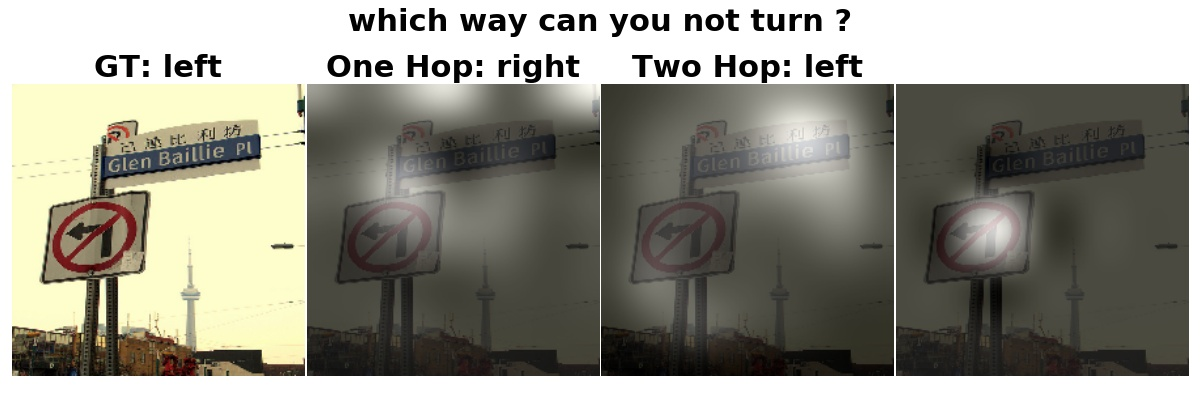
\includegraphics[width=0.5\textwidth]{figures/VQA-DAQUAR_One-Hop_Two-Hop/CO_train2014_000000222383_2223830.jpg}\\
  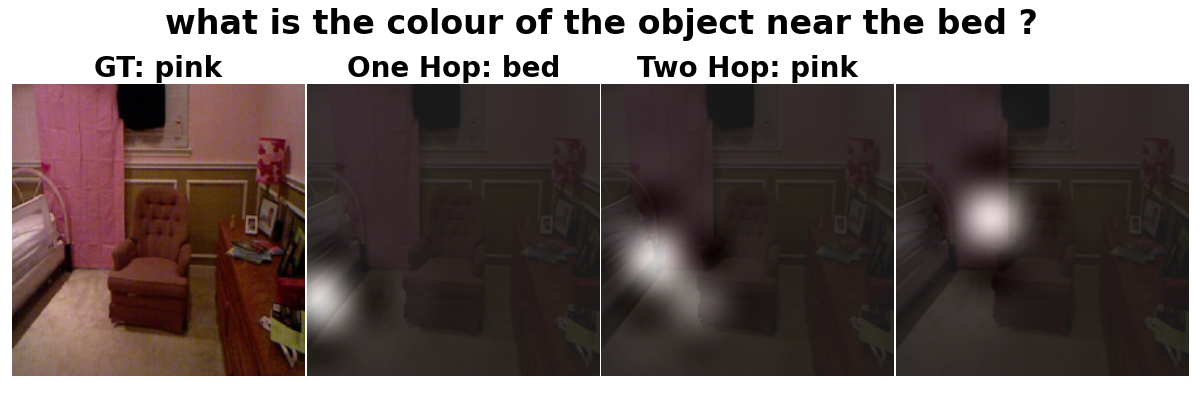
\includegraphics[width=0.5\textwidth]{figures/VQA-DAQUAR_One-Hop_Two-Hop/image1183.png}
  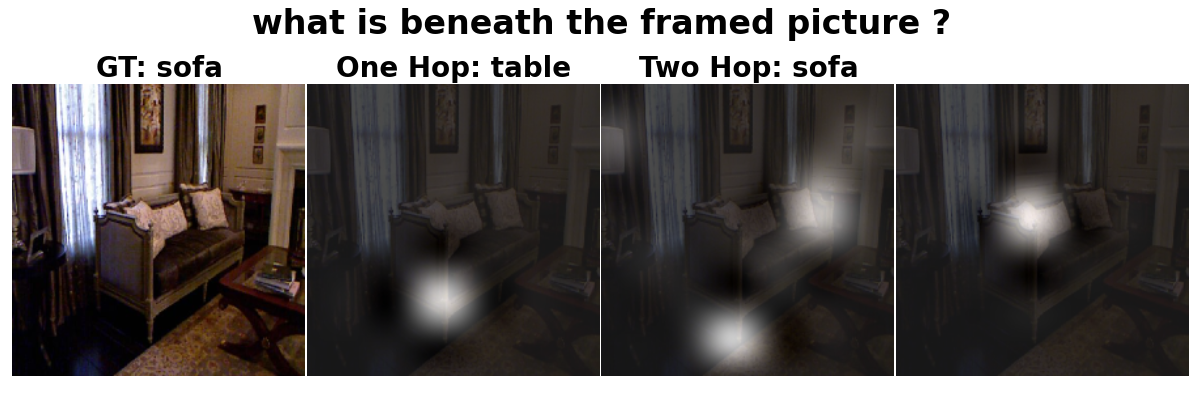
\includegraphics[width=0.5\textwidth]{figures/VQA-DAQUAR_One-Hop_Two-Hop/image1444.png}
\vspace{-0.25in}
\caption{Visualization of the spatial attention weights in the SMem-VQA One-Hop and Two-Hop models on VQA (top row) and DAQUAR (bottom row) datasets. For each image and question pair, we show the original image, the attention weights $W_{att}$ of the One-Hop model, and the two attention weights $W_{att}$ and $W_{att2}$ of the Two-Hop model in order.}\label{fig:2hopVQA}
\vspace{-0.15in}
\end{figure*}
% \vspace{-0.1in}
\subsubsection{Results on VQA}

The VQA dataset is a recent large dataset based on MS COCO~\cite{lin2014microsoft}. We use the full release (V1.0) open-ended dataset, which contains a train set and a val set. Following standard practice, we choose the top 1000 answers in train and val sets as possible prediction answers, and only keep the examples whose answers belong to these 1000 answers as training data. The question vocabulary size is 7477 with the word frequency of at least three.
Because of the larger training size, the embedding dimension is 1000 on the VQA dataset.
We report the test-dev and test-standard results from the VQA evaluation server.
The server evaluation uses the evaluation metric introduced by~\cite{DBLP:journals/corr/AntolALMBZP15}, which gives partial credit to certain synonym answers:
%\begin{equation}
%Acc({\color{red}ans}) = \min\left\{ \frac{\text{\# human that said }{\color{red} ans}}{3},1\right\}
%$Acc({ans}) = \min\left\{ \frac{\text{\# humans that said }{ans}}{3},1\right\}$.
$Acc({ans}) = \min\left\{ (\text{\# humans that said }{ans})/3,1\right\}$.
%\end{equation}


For the attention models, we do not mirror the input image when using the CNN to extract convolutional features, since this might cause confusion about the spatial locations of objects in the input image.
%The input image size for CNN is $224 \times 224$.
The optimization algorithm used is stochastic gradient descent (SGD) with a minibatch of size 50 and momentum of 0.9.
The base learning rate is set to be 0.01 which is halved every six epoches. Regularization, dropout and L2 norm are cross-validated and used. 


%%%%%%%%%%%%%% another candidate table with test-standard
\begin{table}[!t]
\centering
\caption{Test-dev and test-standard results on the Open-Ended VQA dataset (in percentage). Models with ${}^\ast$ use external training data in addition to the VQA dataset.}
\scriptsize
 \begin{tabular}{l || c c c c || c c c c} 
 \hline
 ~ & \multicolumn{4}{c||}{test-dev}  & \multicolumn{4}{c}{test-standard}\\ 
 ~ & \bf{Overall}  & yes/no  & number  & others & \bf{Overall}  & yes/no  & number  & others\\ \hline
 LSTM Q+I~\cite{DBLP:journals/corr/AntolALMBZP15} & 53.74 & 78.94  & 35.24  & 36.42 & 54.06 & -  & -  & -\\ %\hline
 ACK${}^\ast$~\cite{wu2015ask} & 55.72 & 79.23  & 36.13  & 40.08 & 55.98 & 79.05  & 36.10  & 40.61\\ %\hline
 DPPnet${}^\ast$~\cite{noh2015image} & 57.22 & 80.71  & 37.24  & 41.69 & 57.36 & 80.28  & 36.92  & 42.24\\ %\hline
 iBOWIMG~\cite{zhou2015simple} & 55.72 & 76.55  & 35.03  & 42.62 & 55.89 & 76.76  & 34.98  & 42.62\\ \hline 
 SMem-VQA One-Hop & 56.56 & 78.98 & 35.93  & 42.09 & - & -  & -  & -\\ %\hline   
 SMem-VQA Two-Hop & \textbf{57.99} & \textbf{80.87}  & \textbf{37.32}  & \textbf{43.12} & \textbf{58.24} & \textbf{80.8}  & \textbf{37.53}  & \textbf{43.48}\\ \hline 
 \end{tabular}
\label{fig:baseline2}
\vspace{-0.15in}
\end{table}

For the VQA dataset, we use the simple iBOWIMG model in~\cite{zhou2015simple} as one baseline model, which beats most existing VQA models currently on arxiv.org. We also compare to two models in~\cite{wu2015ask}\cite{noh2015image} which have comparable or better results to the iBOWIMG model. These three baseline models as well the best model in VQA dataset paper~\cite{DBLP:journals/corr/AntolALMBZP15} are listed in the following:\\
%\noindent
{$\bullet$} {\bf{LSTM Q+I}}~\cite{DBLP:journals/corr/AntolALMBZP15}: uses the element-wise multiplication of the LSTM encoding of the question and the image feature vector to predict the answer. This is the best model in the VQA dataset paper.\\
{$\bullet$} {\bf{ACK}}~\cite{wu2015ask}: shows the image attribute features, the generated image caption and relevant external knowledge from knowledge base to the LSTM at the first time step, and the question in the remaining time steps to predict the answer.\\
{$\bullet$} {\bf{DPPnet}}~\cite{noh2015image}: uses the Gated Recurrent Unit (GRU) representation of question to predict certain parameters for a CNN classification network. They pre-train the GRU for question representation on a large-scale text corpus to improve the GRU generalization performance.\\
{$\bullet$} {\bf{iBOWIMG}}~\cite{zhou2015simple}: concatenates the BOW question representation with image feature (GoogLeNet), and uses a softmax classification to predict the answer. 

The overall accuracy and per-answer category accuracy for our SMem-VQA models and the four baseline models on VQA dataset are shown in Tab.~\ref{fig:baseline2}. From the table, we can see that the SMem-VQA One-Hop model obtains slightly better results compared to the iBOWIMG model. However, the SMem-VQA Two-Hop model achieves an improvement of 2.27\% on test-dev and 2.35\% on test-standard compared to the iBOWIMG model, demonstrating the value of spatial attention. The SMem-VQA Two-Hop model also shows best performance in the per-answer category accuracy. 
The SMem-VQA Two-Hop model has slightly better result than the DPPnet model. 
The DPPnet model uses a large-scale text corpus to pre-train the Gated Recurrent Unit (GRU) network for question representation.
Similar pre-training work on extra data to improve model accuracy has been done in~\cite{venugopalan2014translating}.
Considering the fact that our model does not use extra data to pre-train the word embeddings, its results are very competitive.
We also experiment with adding a third hop into our model on the VQA dataset, but the result does not improve further.

The attention weights visualization examples for the SMem-VQA One-Hop and Two-Hop models on the VQA dataset are shown in Fig.~\ref{fig:2hopVQA} (top row). From the visualization, we can see that the two-hop model collects supplementary evidence for inferring the answer, which may be necessary to achieve an improvement on these complicated real-world datasets. We also visualize the fine-grained alignment in the first hop of our SMem-VQA Two-Hop model in Fig.~\ref{fig:VQA_hop1Atten_wordAtten}. 
%through visualizing the attention weights and the correlation value vector from the correlation matrix $C$ for the location with highest attention weight
The correlation vector values (blue bars) measure the correlation between image regions and each word vector in the question. Higher values indicate stronger correlation of that particular word with the specific location's image features. We observe that the fine-grained visual evidence collected using each local word vector, together with the global visual evidence from the whole question, complement each other to infer the correct answer for the given image and question, as shown in Fig.~\ref{fig:concept}.


%%%%%%%%%%% figure
\begin{figure*}[t]
  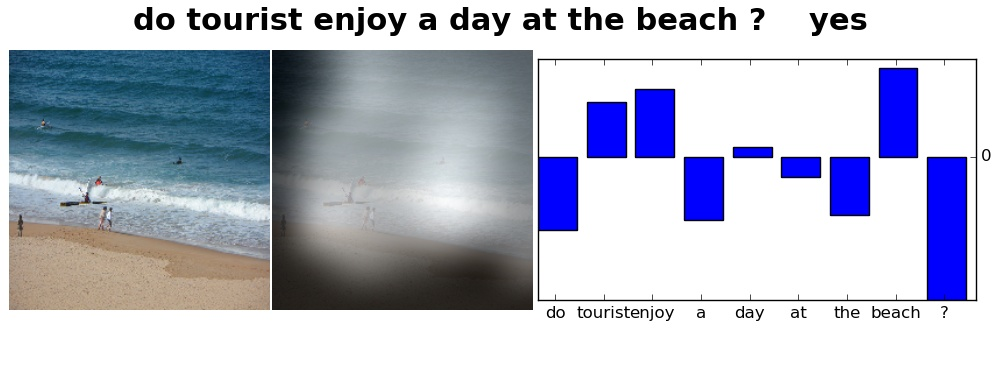
\includegraphics[width=0.5\textwidth]{figures/word_atten/COCO_val2014_000000540932_5409320.jpg}
  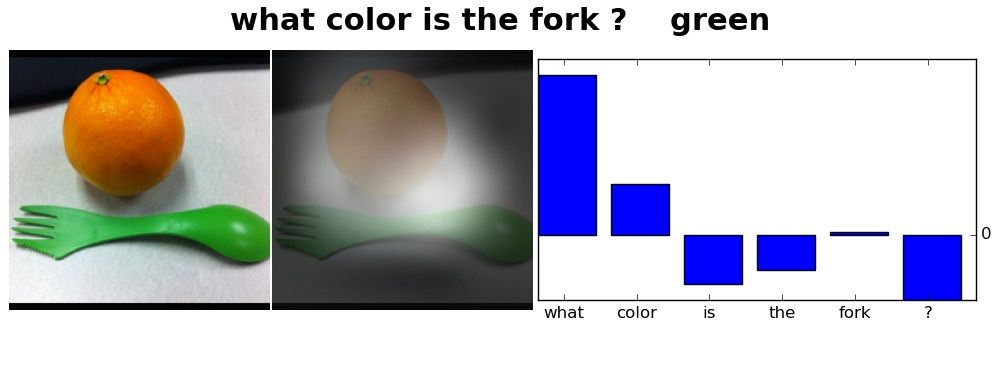
\includegraphics[width=0.5\textwidth]{figures/word_atten/COCO_val2014_000000563730_5637302.jpg}\\
  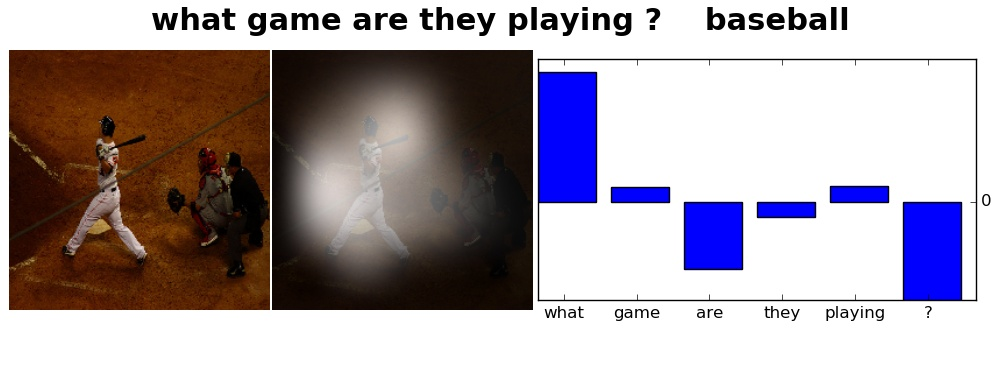
\includegraphics[width=0.5\textwidth]{figures/word_atten/COCO_val2014_000000576875_5768752.jpg}
  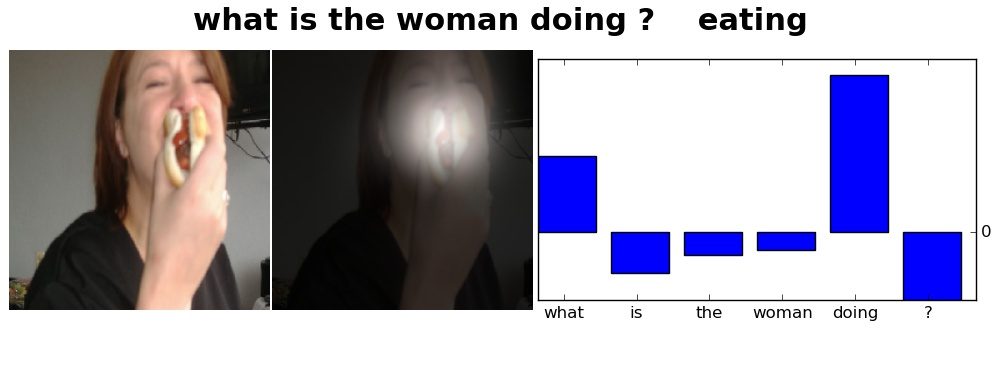
\includegraphics[width=0.5\textwidth]{figures/word_atten/COCO_val2014_000000567340_5673401.jpg}
\vspace{-0.3in}
\caption{
Visualization of the original image (left), the spatial attention weights $W_{att}$ in the first hop (middle) and one correlation vector from the correlation matrix $C$ for the location with highest attention weight in the SMem-VQA Two-Hop model on the VQA dataset.
Higher values in the correlation  vector indicate  stronger correlation of that word with the chosen location's image features.}
\label{fig:VQA_hop1Atten_wordAtten}
\vspace{-0.15in}
\end{figure*}




 







\section{Conclusion}
We propose a new method to train neural samplers for given distributions, together with a new SteinGAN method for generative adversarial training. 
Future directions involve more applications and theoretical understandings for training neural samplers. 

\newpage\clearpage
\bibliographystyle{iclr2016_conference}
{\small
\bibliography{bibrkhs_stein}
}

%\newpage
\appendix
\begin{figure}[h]
\centering
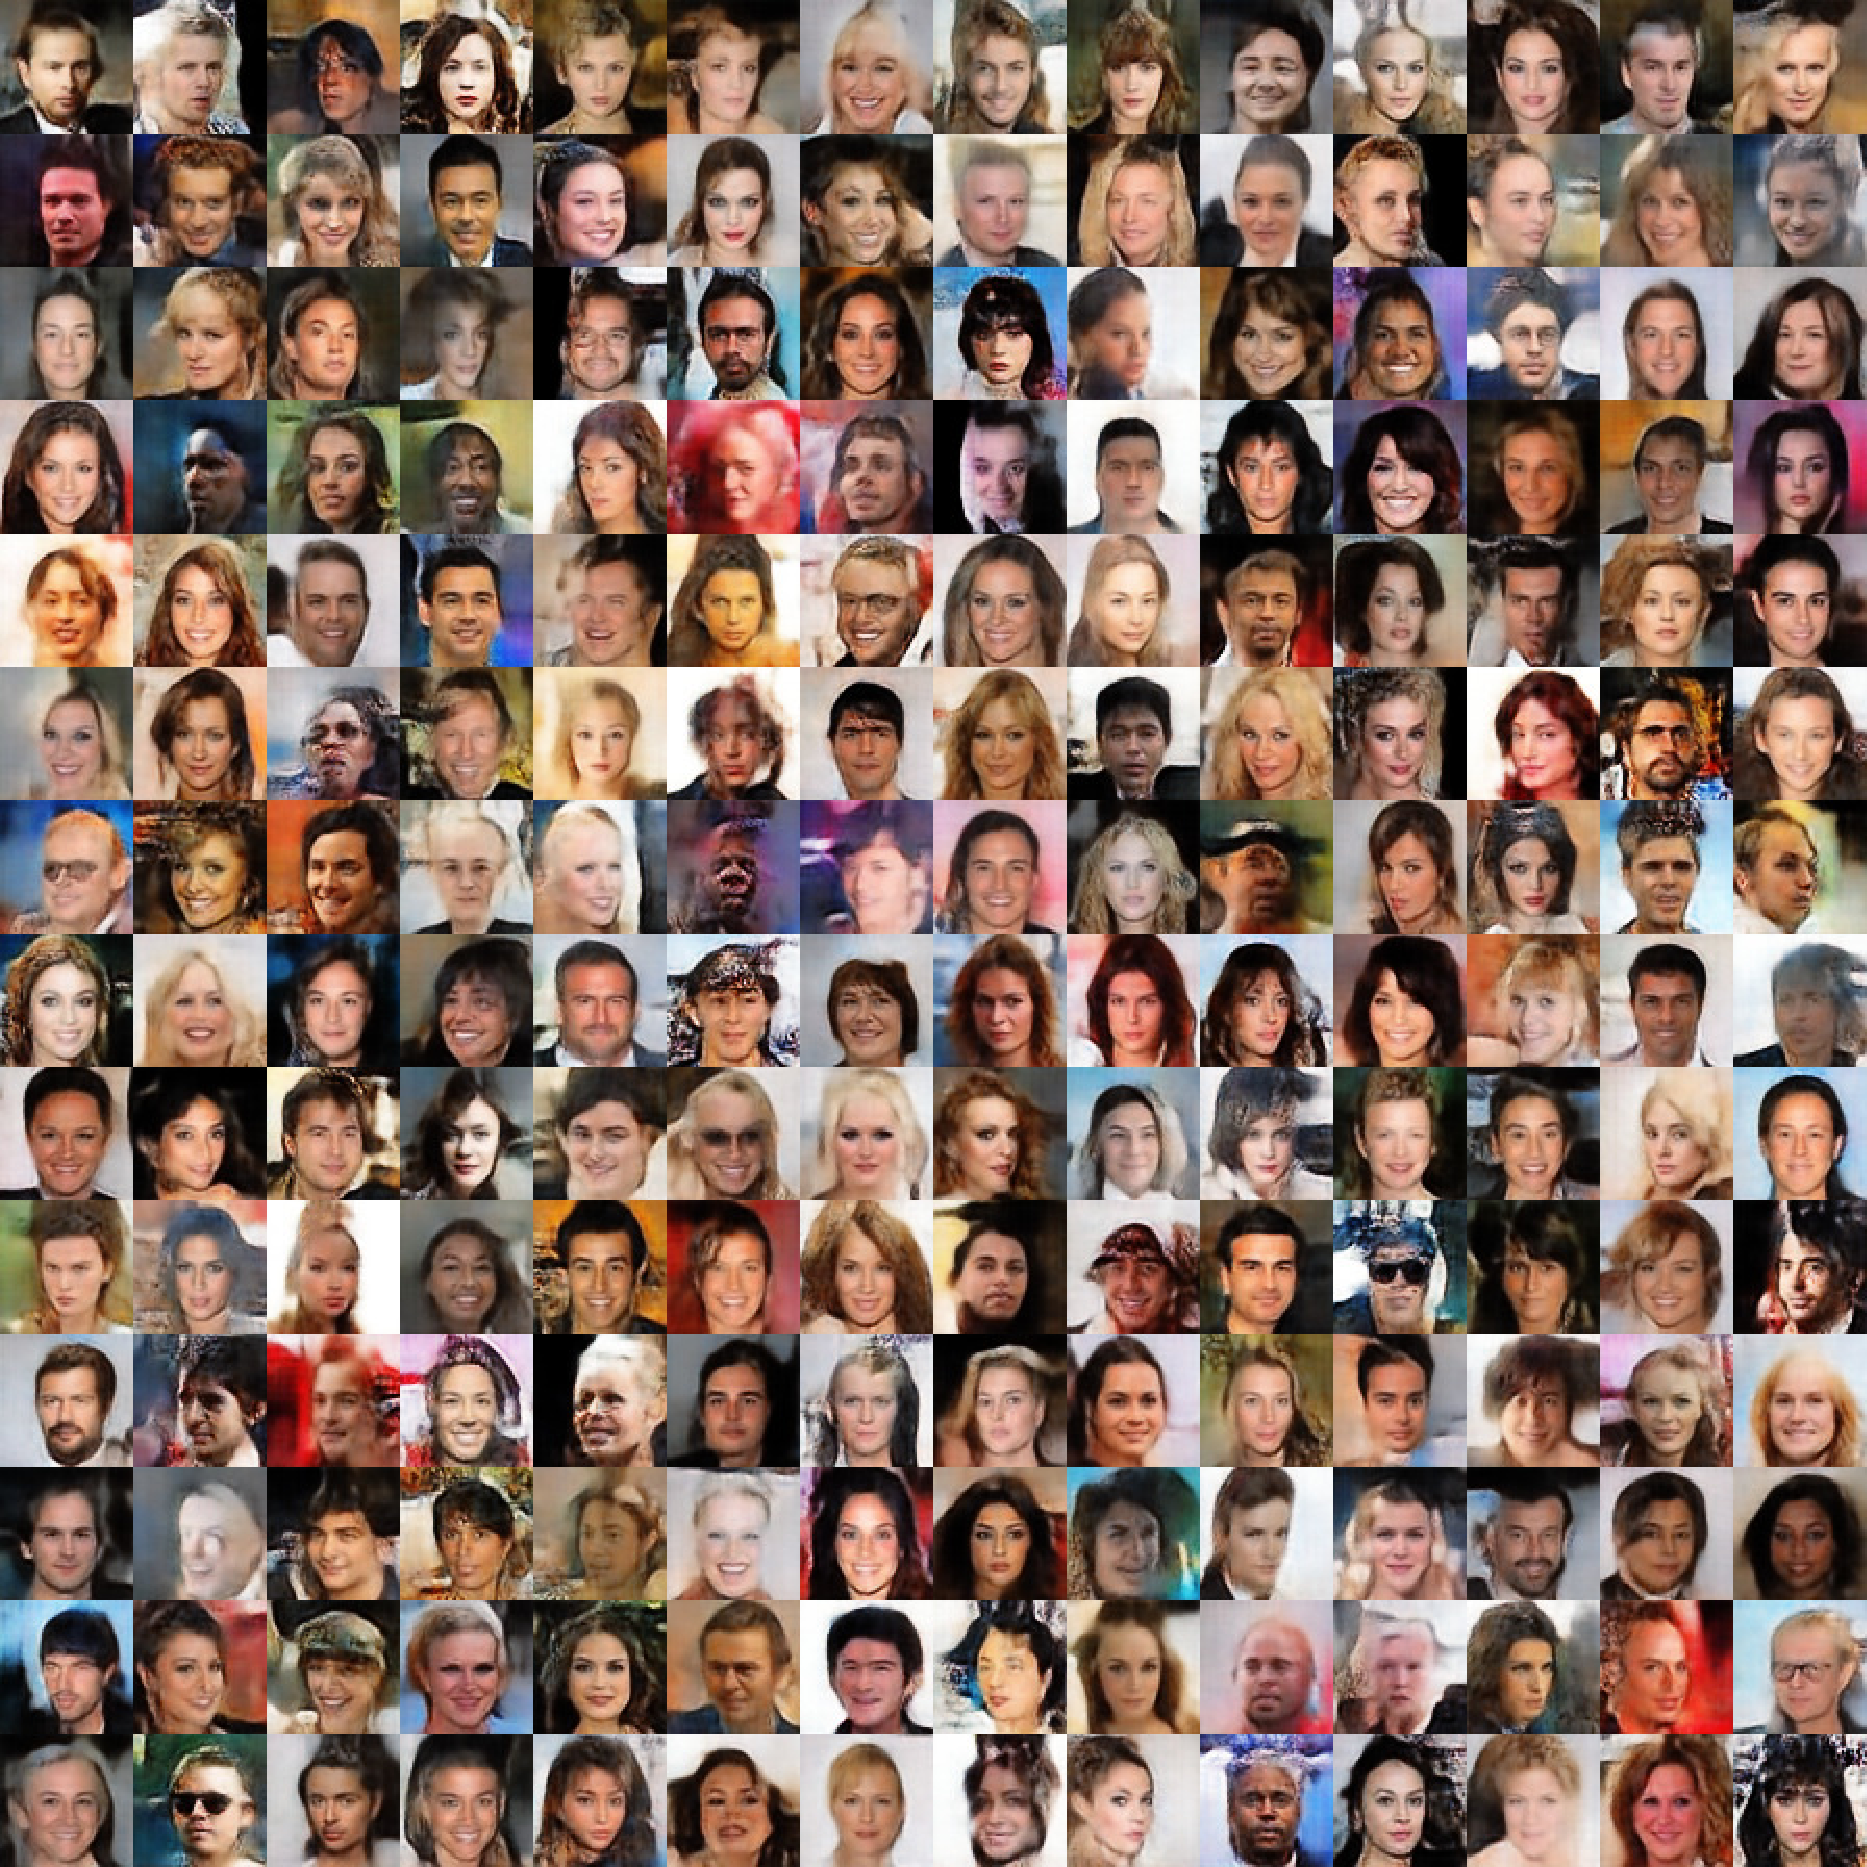
\includegraphics[width=0.9\textwidth]{\dilinfig/faces/vgd_gan-20.pdf}  
\caption{More images generated by SteinGAN on CelebA.}
\label{fig:facemore}
\end{figure}


\end{document}
